%% LyX 2.3.3 created this file.  For more info, see http://www.lyx.org/.
%% Do not edit unless you really know what you are doing.
\documentclass[english]{article}
\usepackage[T1]{fontenc}
\usepackage[latin9]{inputenc}
\usepackage{geometry}
\geometry{verbose,tmargin=1in,bmargin=1in,lmargin=1in,rmargin=1in}
\usepackage{babel}
\usepackage{float}
\usepackage{hyperref}
\hypersetup{
    colorlinks=true,
    linkcolor=blue,
    filecolor=magenta,      
    urlcolor=cyan,
}

\makeatletter
%%%%%%%%%%%%%%%%%%%%%%%%%%%%%% User specified LaTeX commands.
\usepackage{bookmark}
\usepackage[sc]{mathpazo}
\usepackage[T1]{fontenc}
\usepackage{bookmark}

% Some math operators
\renewcommand{\epsilon}{\varepsilon}

\usepackage{graphicx}
\hypersetup{urlcolor=blue}

\raggedbottom

%\setlength{\parindent}{1em}

\makeatother

\begin{document}
\title{Experiments Using Facebook Chatbots }
\author{Ricardo Ruiz\thanks{Stanford Graduate School Of Business, email: Ricardo.Ruiz@stanford.edu}}
\date{\today}
\maketitle
\begin{abstract}
The plan is to make this document a blog post that describes the process
of running both adaptive and non-adaptive experiments using the Facebook
chatbot, Chatfuel. \newpage{}
\end{abstract}

\section{What are Chatbots?}

Chatbots are AI or non-AI software that can simulate a conversation
with a user through messaging applications. You may have interacted
with them before through customer service bots, e-commerce chatbots,
or virtual assistants(Siri). In our case, we will cover the chatbot
software, Chatfuel, that allows us to create non-AI chatbots using
Facebook messenger. Chatfuel provides some AI capabilities; however, we will not cover them in this article. This chatbot platform
is incredibly flexible, allowing us to create branching logic, export
data, and connect with external services, all while writing no code
and building the entire bot by using the provided user interface.
The benefits of chatbots in the experimental context include the ease
of use for the user, the familiarity of the chatting platform to the
user, the ease of advertisement, and the ease of data collection.

\section{The User Experience }

After being directed to your chatbot through either a Facebook advertisement or some other distribution mechanism, the user will be greeted by a welcome message that you, the researcher, create. Below we show the interactions between the Misinformation chatbot and a user. As you can see, users interact with the chatbot in two ways, either through a text response or by pressing a button. 

\begin{figure}[H]
\center{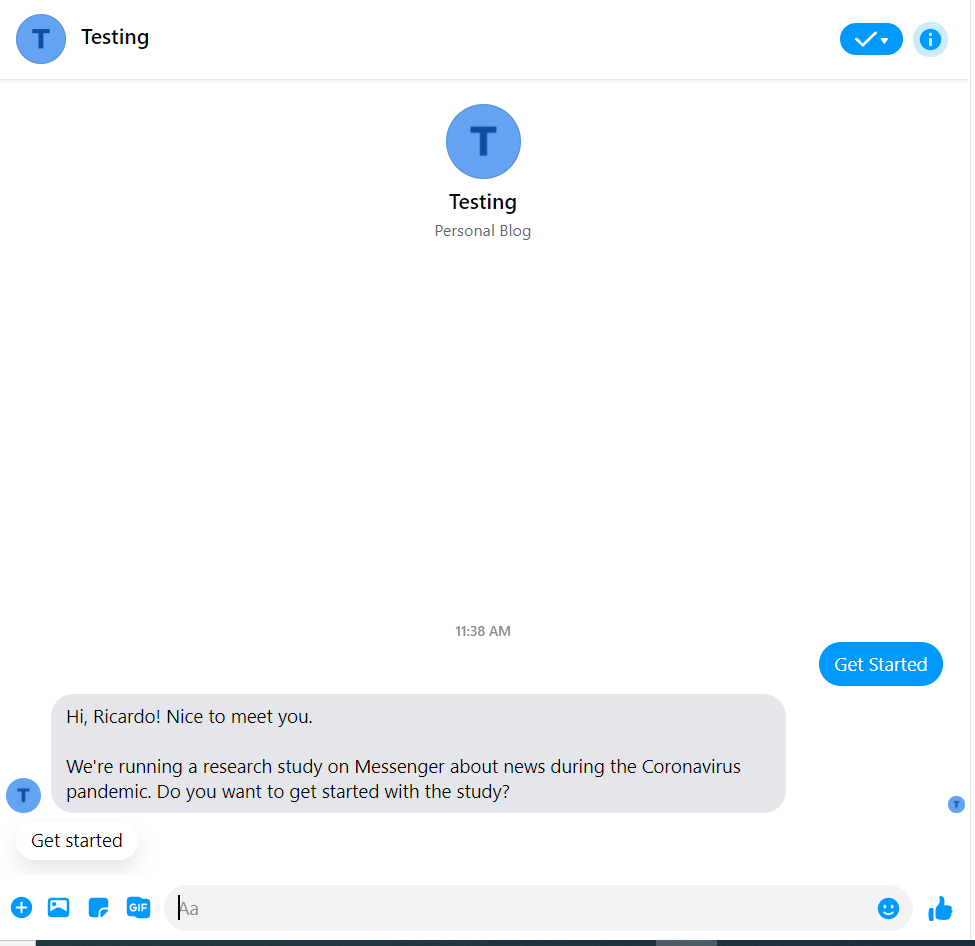
\includegraphics[scale=0.4]{assets/welcome_message.PNG}}

\caption{Chatfuel: Welcome Message}
\end{figure}

\begin{figure}[H]
\center{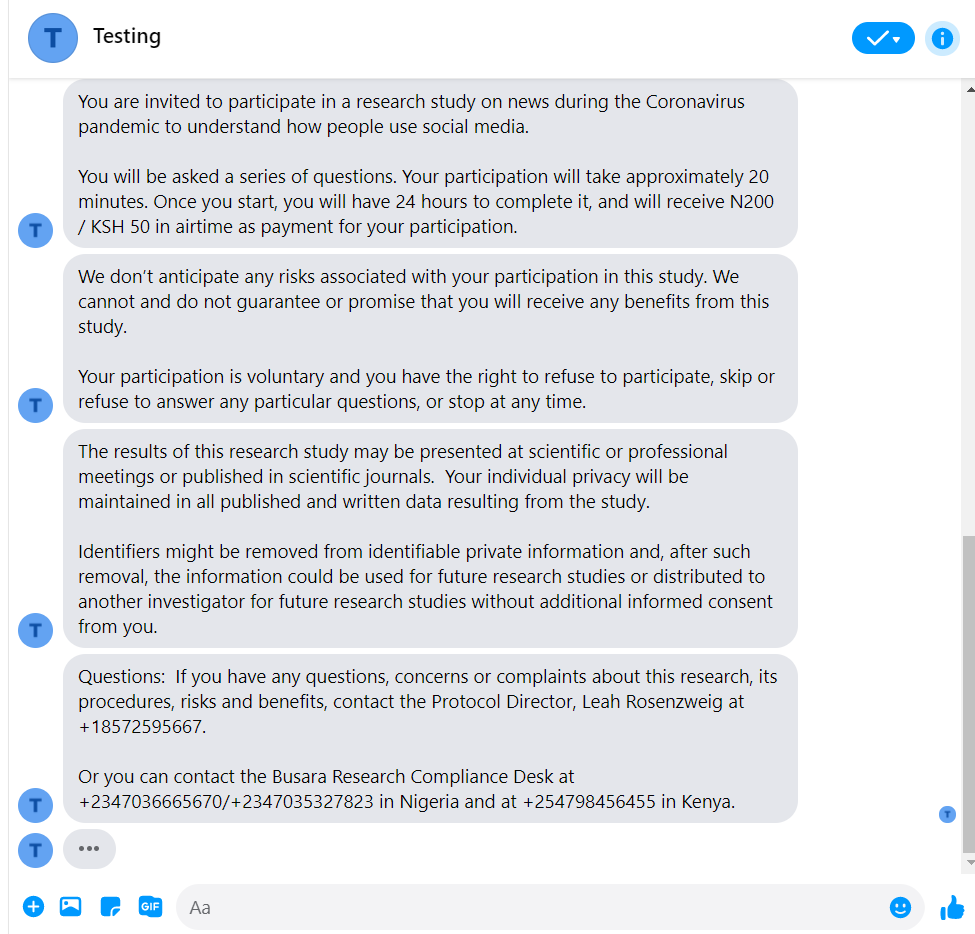
\includegraphics[scale=0.4]{assets/ellipse.PNG}}

\caption{Chatfuel: Ellipse}
\end{figure}

\begin{figure}[H]
\center{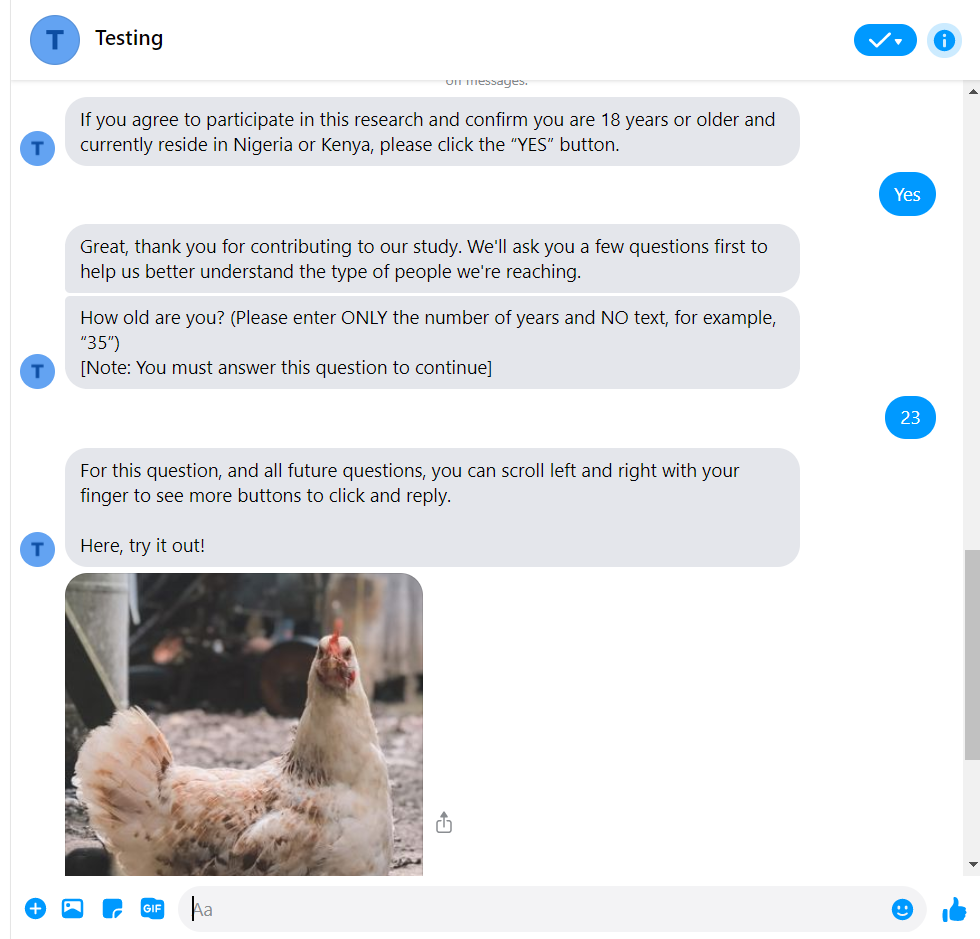
\includegraphics[scale=0.4]{assets/more_chats.PNG}}

\caption{Chatfuel: More}
\end{figure}


\section{The Researcher's Perspective }

\subsection{Before the Experiment}
\subsubsection{ Creating the Bot}
\begin{enumerate}
\item \textbf{Create Facebook account}

\item \textbf{Go to the Chatfuel \href{http://Chatfuel.com}{website}, and create an account}

\begin{figure}[H]
\center{\includegraphics[scale=0.4]{assets/Chatfuel_signup.PNG}}

\caption{Chatfuel: Sign Up}
\end{figure}

\item \textbf{create a Facebook page to host chatbot}\newline

This will be the page that individuals see when messaging with the chatbot. For example, this is the \href{https://www.facebook.com/socialimpactresearchlab/}{page},
we used for the misinformation experiment.

\begin{figure}[H]
\center{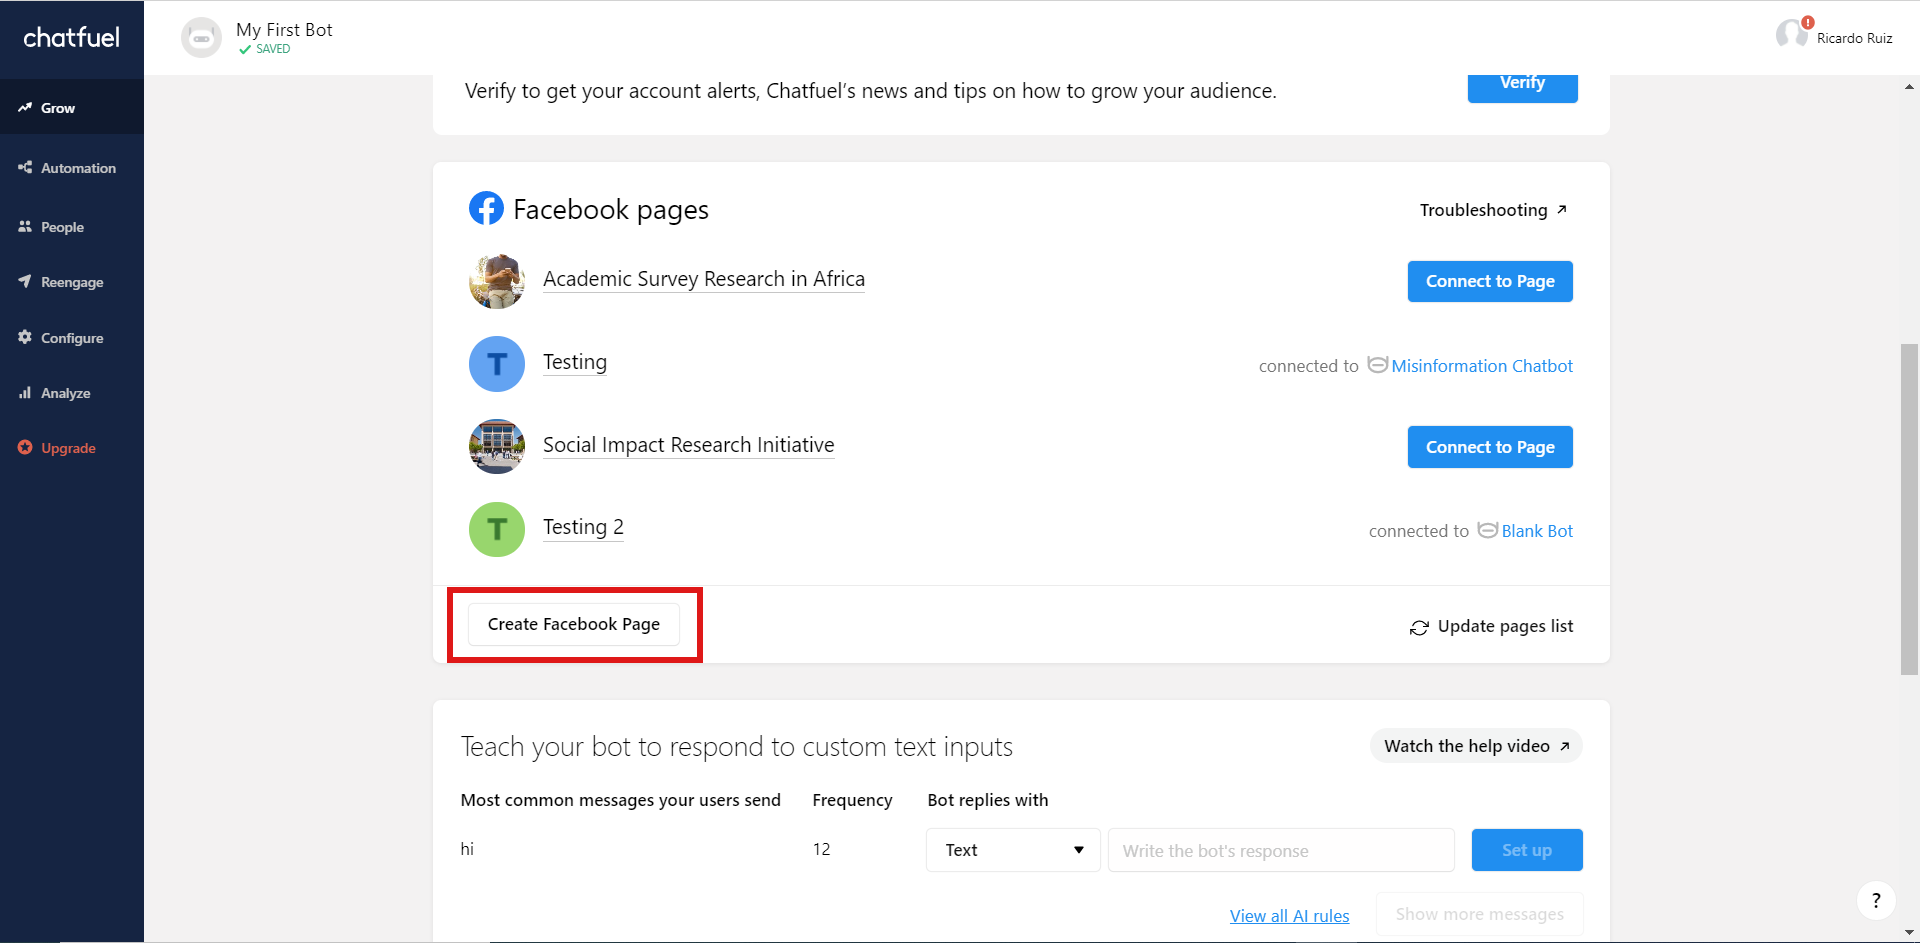
\includegraphics[scale=0.4]{assets/create_button_redbox.PNG}}

\caption{Chatfuel: Create Facebook Page}
\end{figure}

\item \textbf{create blank bot}\newline

This will be the starting point for our chatbot. To make a blank
bot go to the Chatfuel dashboard and click on the blue add blank
bot button located at the top right of the page.

\begin{figure}[H]
\center{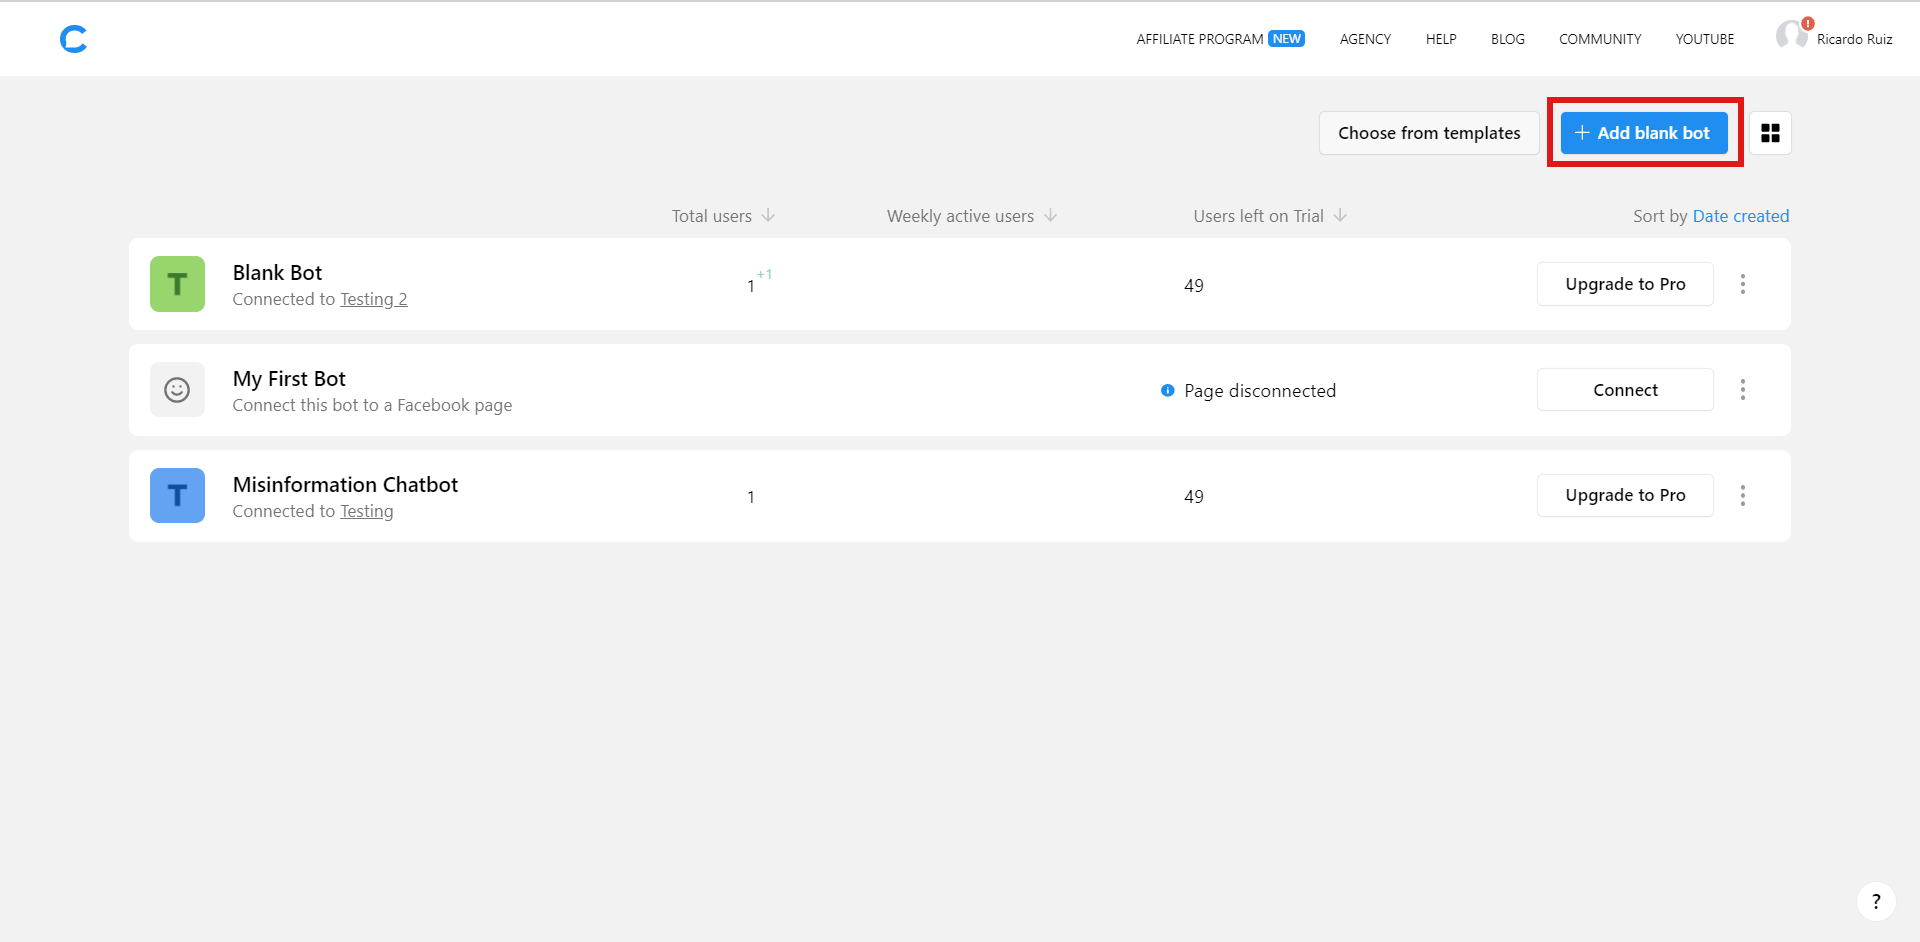
\includegraphics[scale=0.4]{assets/create_blank_bot_redbox.PNG}}

\caption{Chatfuel: Create Blank Bot}
\end{figure}

\begin{figure}[H]
\center{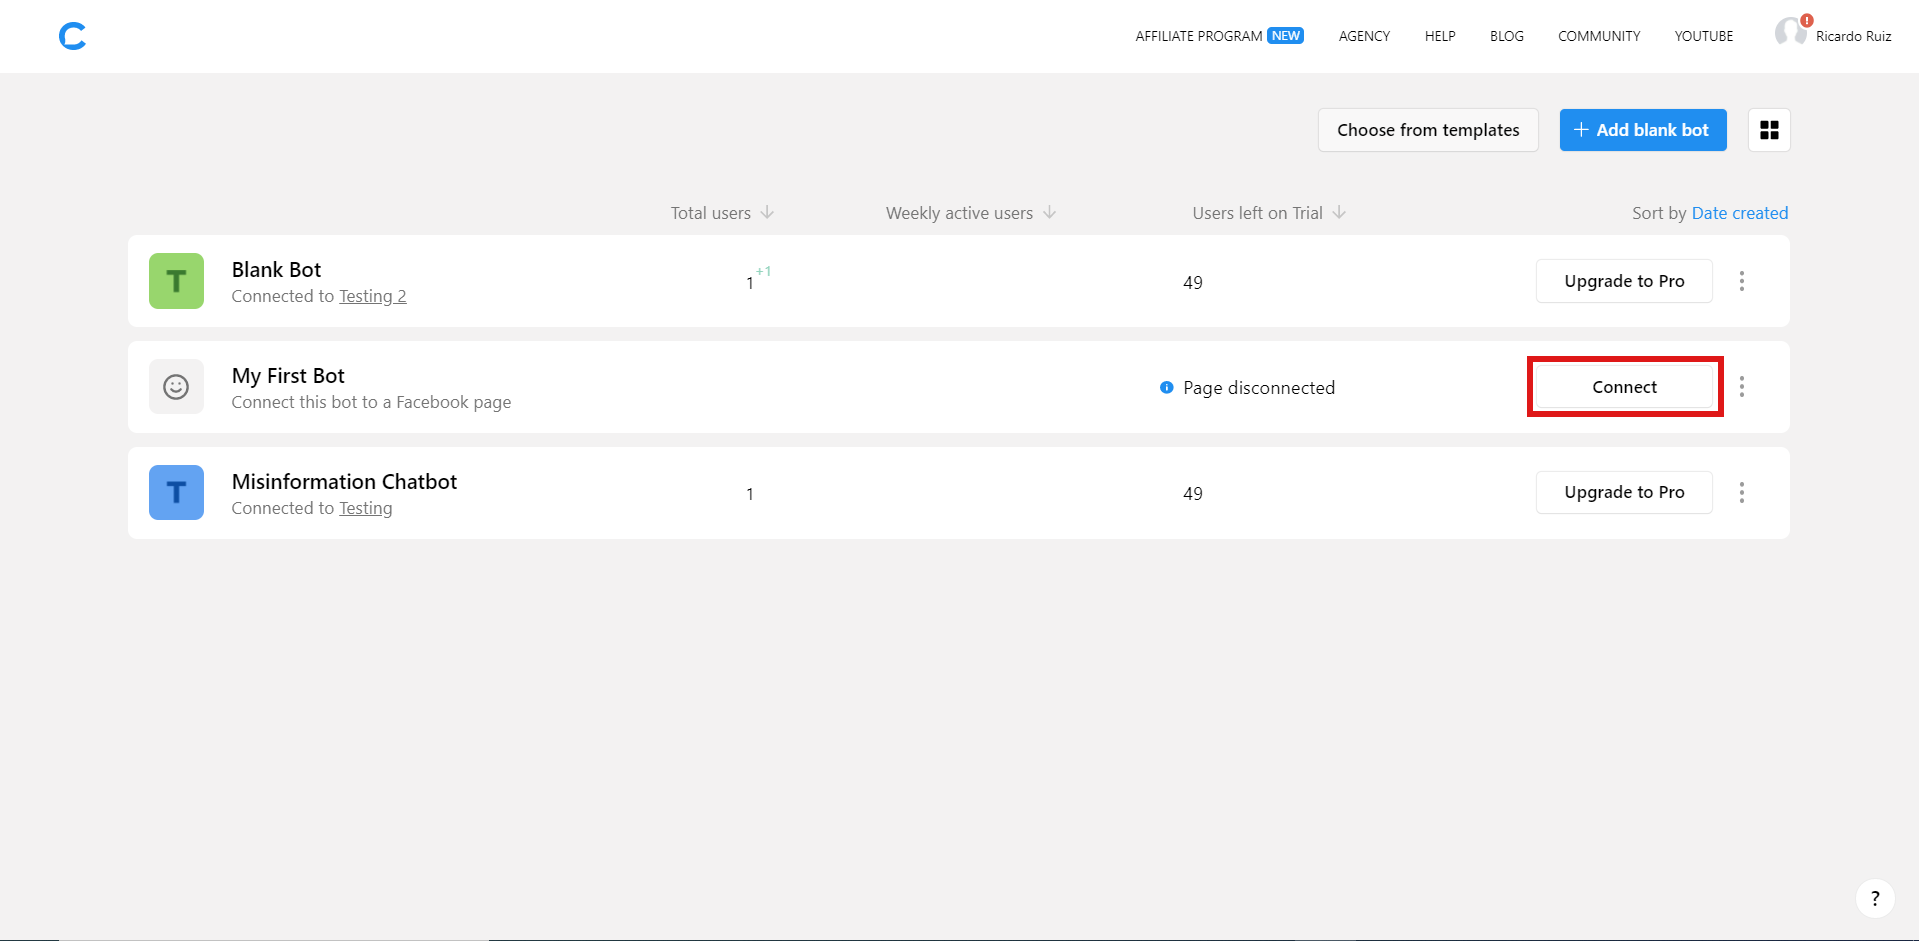
\includegraphics[scale=0.4]{assets/connect_to_page_redbox.PNG}}

\caption{Chatfuel: Dashboard}
\end{figure}

\item \textbf{Connect chatbot to Facebook page}\newline

In the chatbot's grow tab, you will see the connect to page button; choose the Facebook page you wish to connect the chatbot to.


\begin{figure}[H]
\center{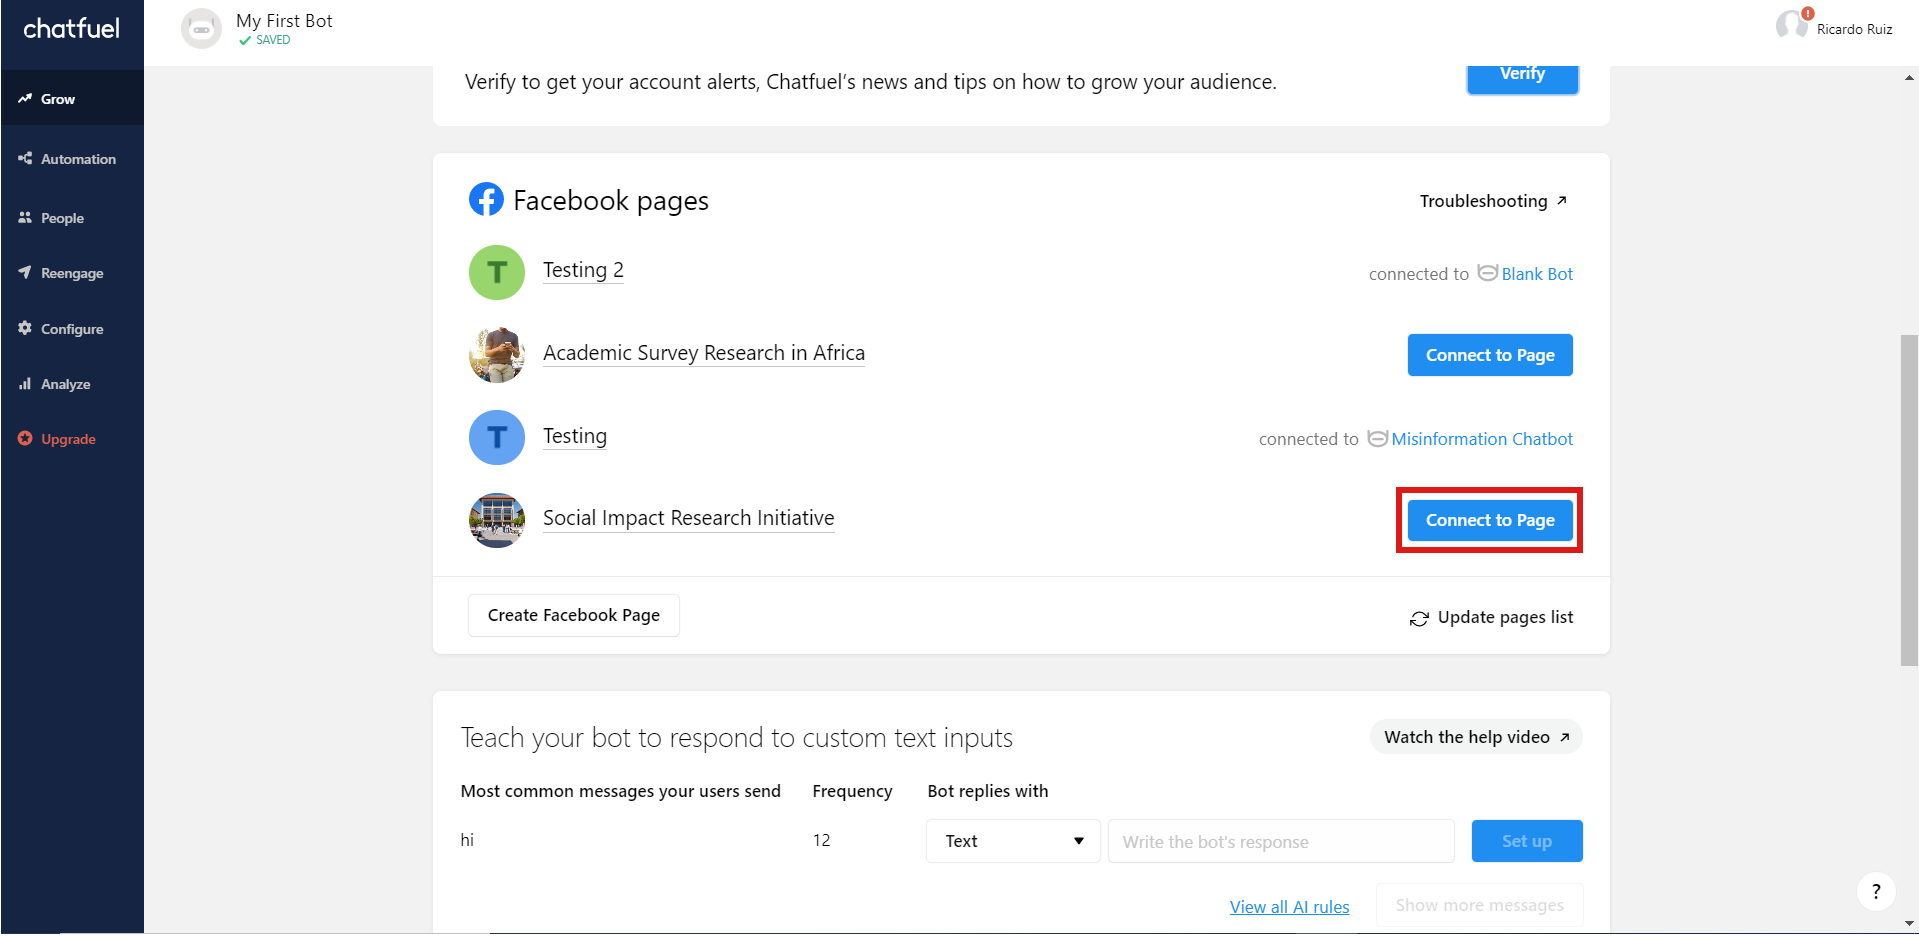
\includegraphics[scale=0.4]{assets/connect_button_redbox.PNG}}

\caption{Chatfuel: Connecting the Bot to the Facebook Page}
\end{figure}


\end{enumerate}



\subsubsection{Setting up the Bot}

Now we are ready to begin setting up the chatbot. You can build it
using either Flows or Blocks. We will go over using Blocks to setup
the chatbot. 

\begin{figure}[H]
\center{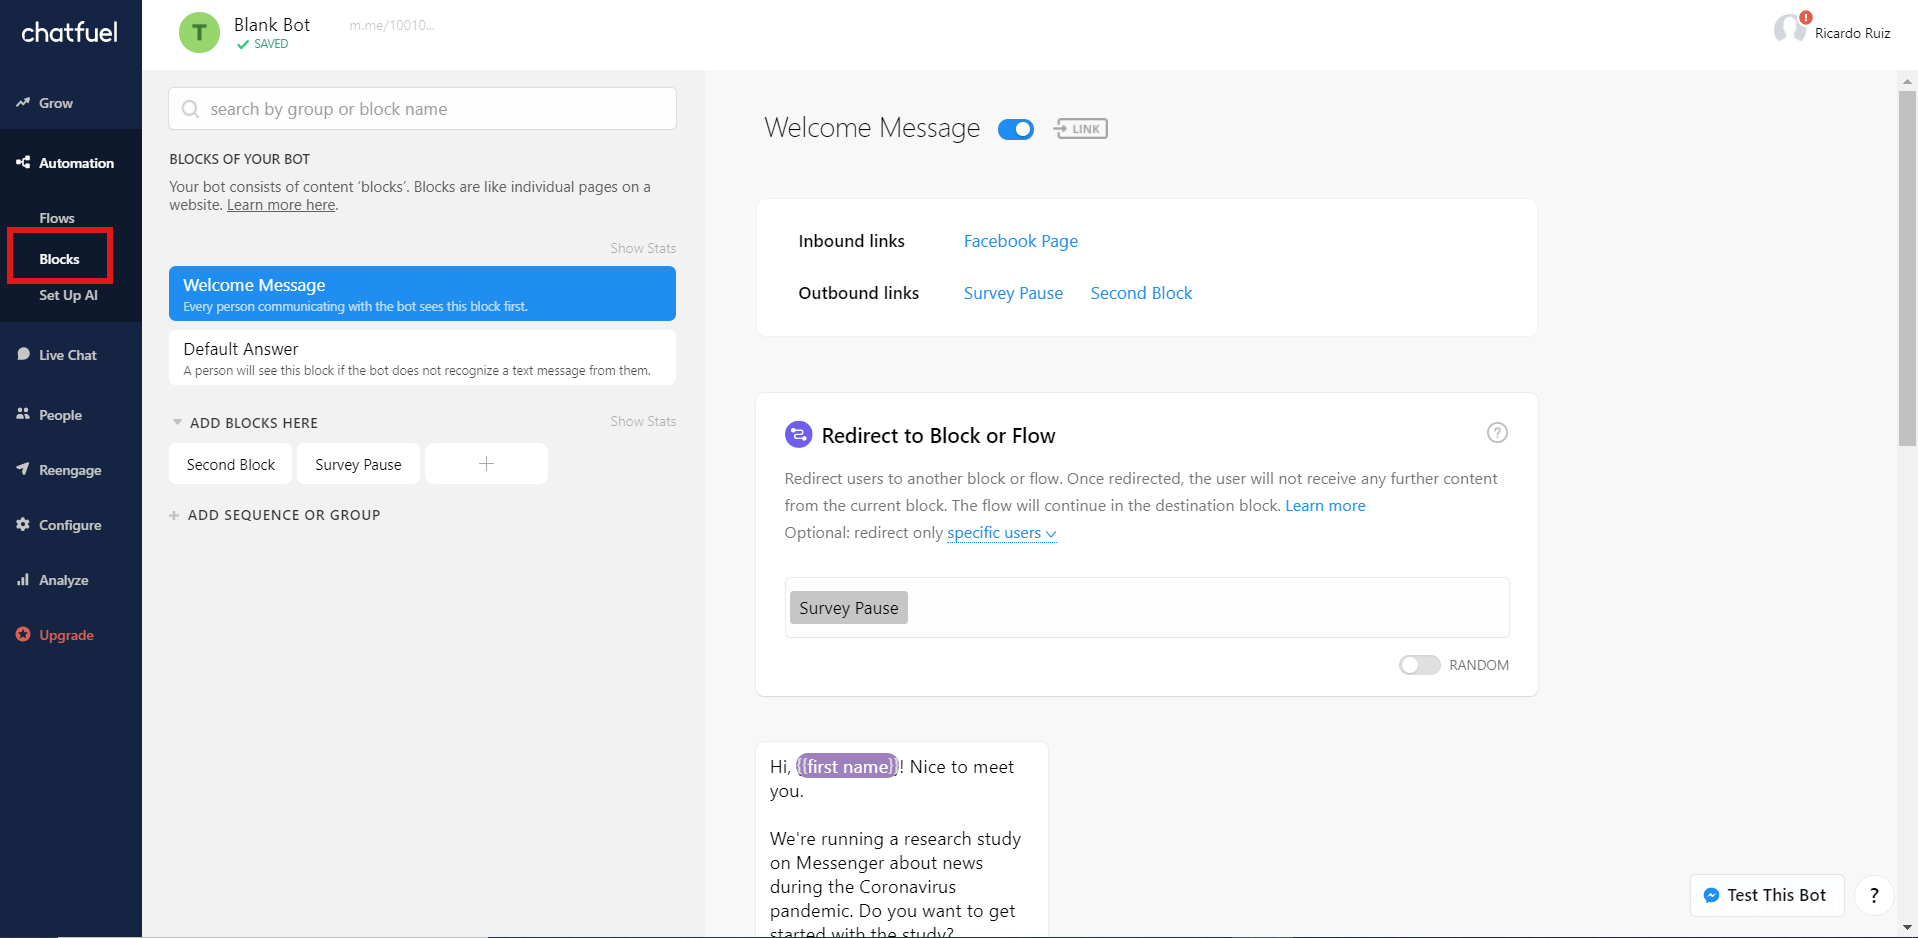
\includegraphics[scale=0.4]{assets/blocks_redbox.PNG}}

\caption{Chatfuel: Blocks}
\end{figure}

\begin{enumerate}
    \item \textbf{set up the Welcome Message and the Default Answer}
    
 The Welcome message will be the first message that an individual sees when they begin interacting with the chatbot, and the Default Answer will be the response given by the bot when it has no other response to give; this will be the response people see once they have reached the end of the survey, and they attempt to interact with the chatbot. 
 
    \item \textbf{Set up block link} \newline 
 
 To see how a user will experience the chatbot, we need to set up a block reference by clicking the link button, Figure 10. Now we will be able to interact with the chatbot from this block by clicking the link that appears in the center of your Chatfuel dashboard. Figure 11.
 
 \begin{figure}[H]
\center{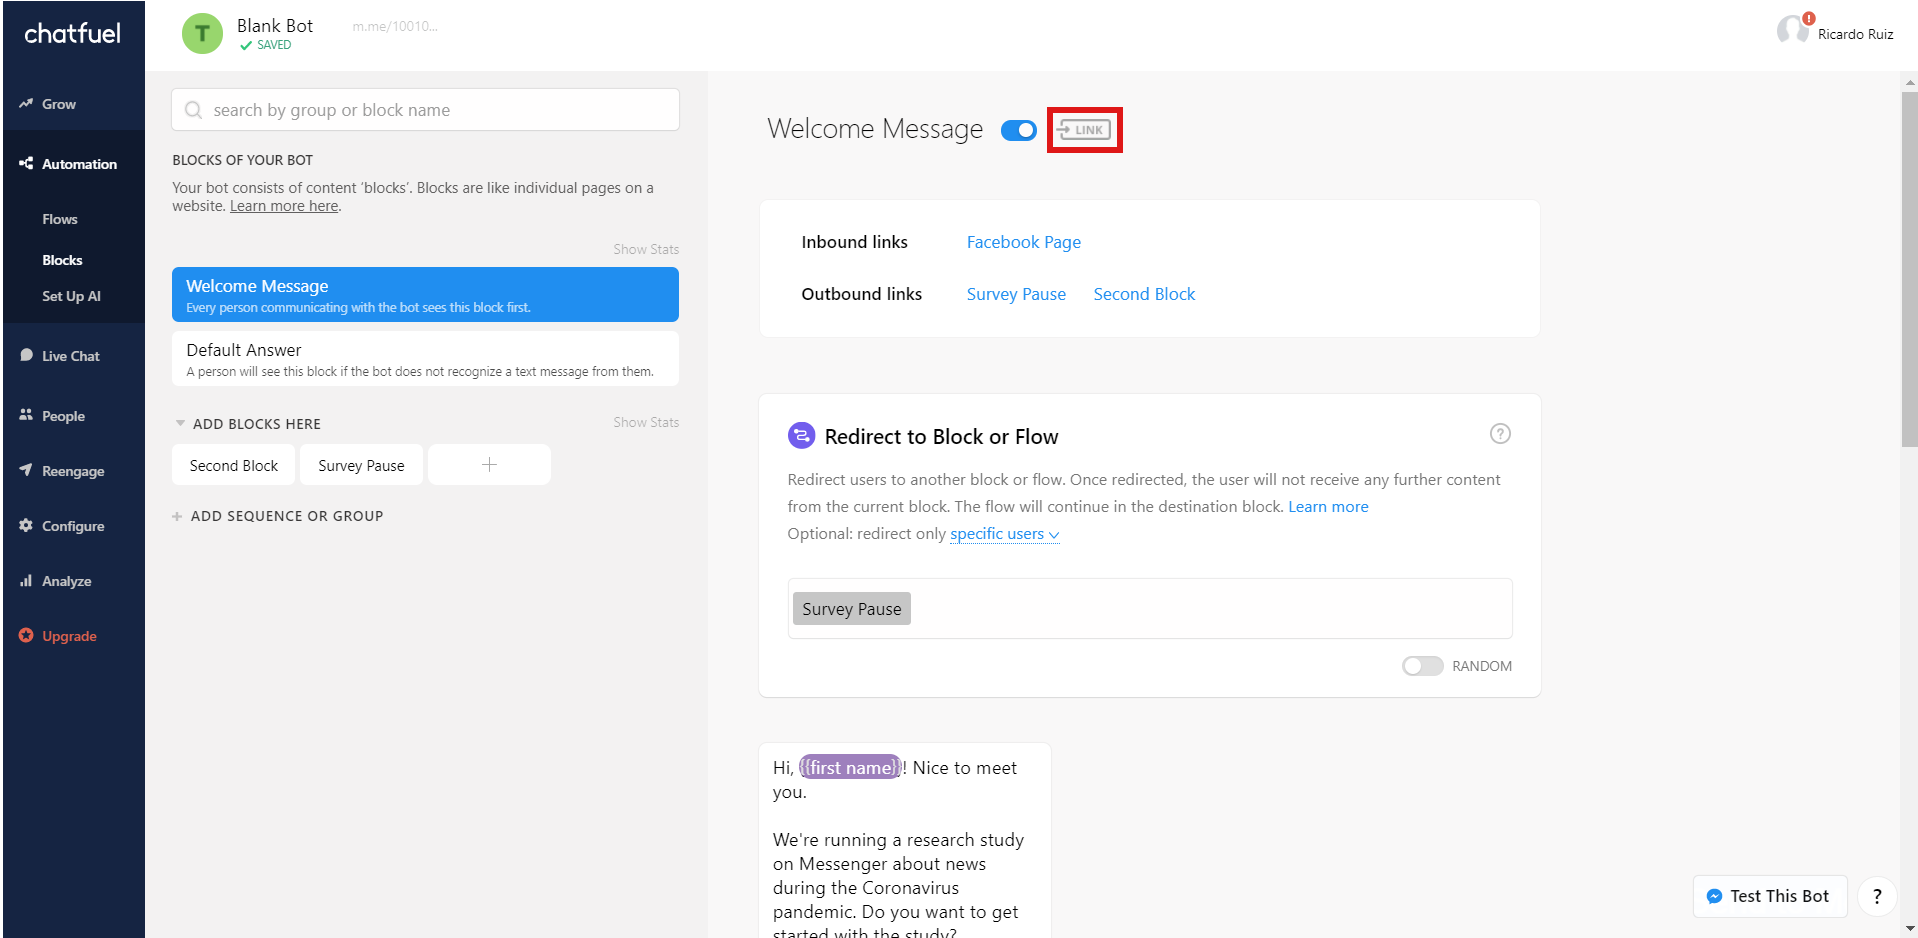
\includegraphics[scale=0.4]{assets/link_redbox.PNG}}

\caption{Chatfuel: Create Block Link}
\end{figure}

\begin{figure}[H]
\center{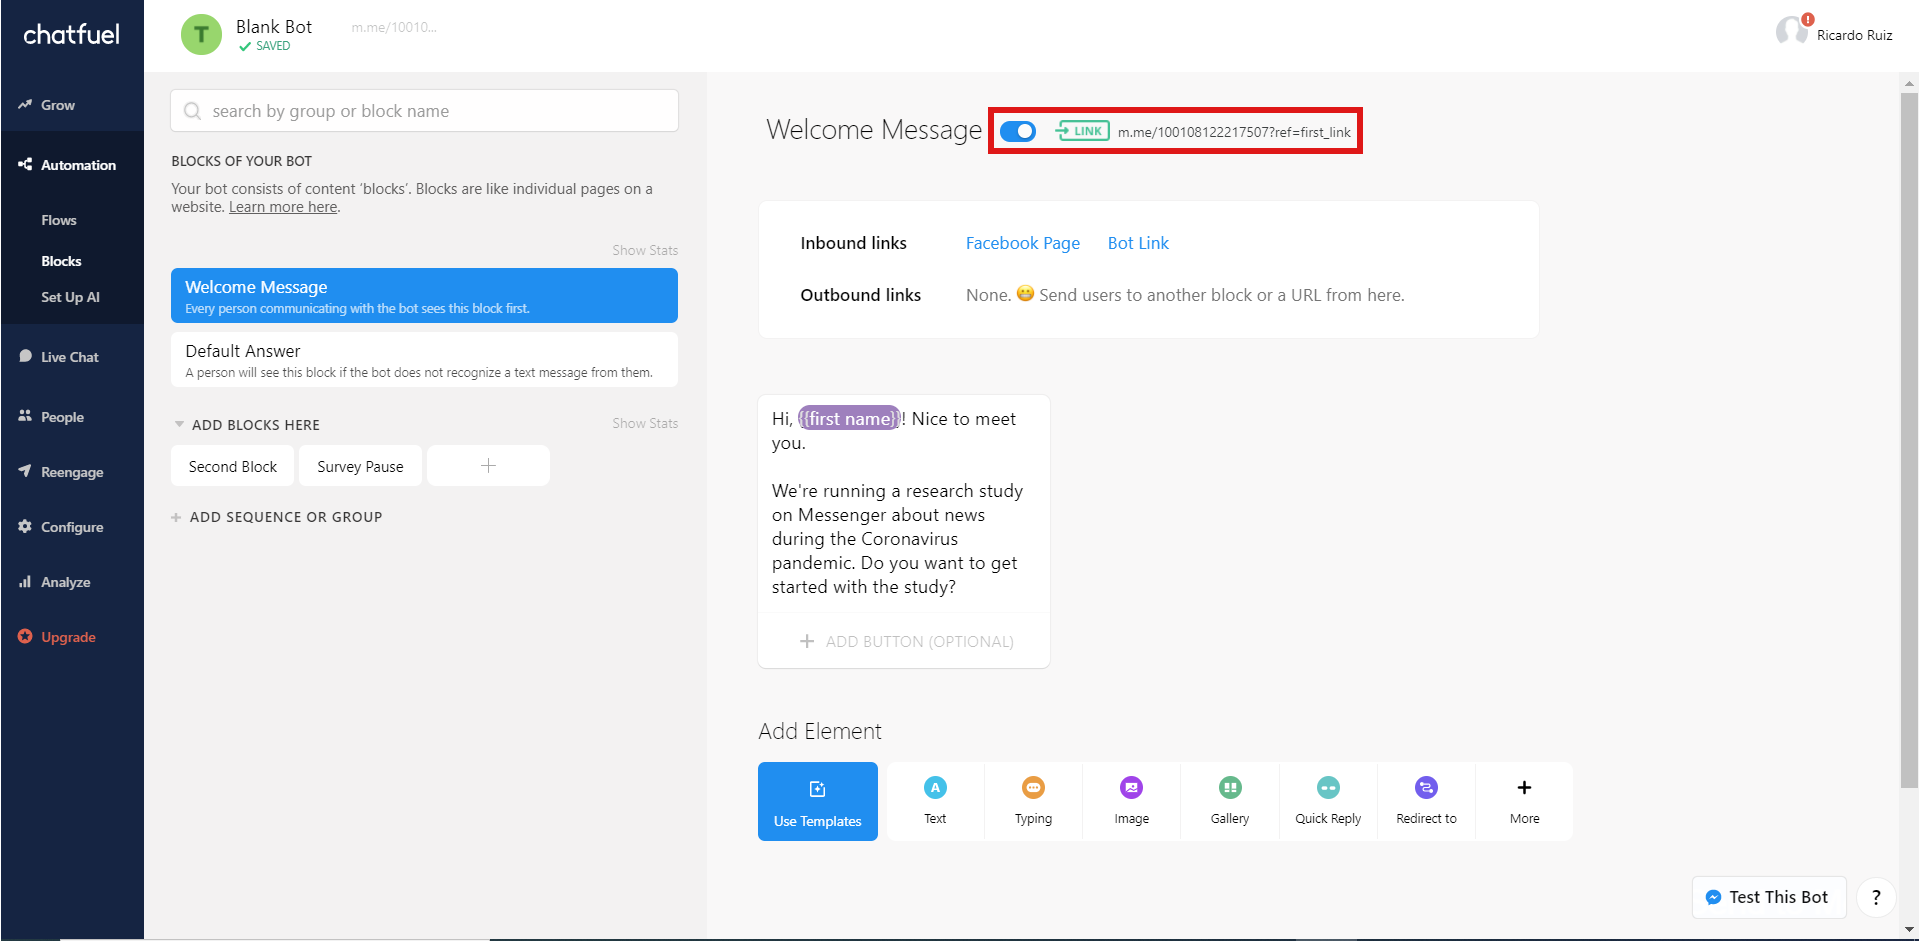
\includegraphics[scale=0.4]{assets/link_click_redbox.PNG}}

\caption{Chatfuel: Block Link}
\end{figure}


 
\end{enumerate}


\newpage 
\subsubsection{The Basics}

We will now go over some of the basic operations and functions that
are available within Chatfuel. 

\subsubsection*{Deleting Cards }

The Individual sections that make up a block are called cards. The
following figure show how to delete them.

\begin{figure}[H]
\center{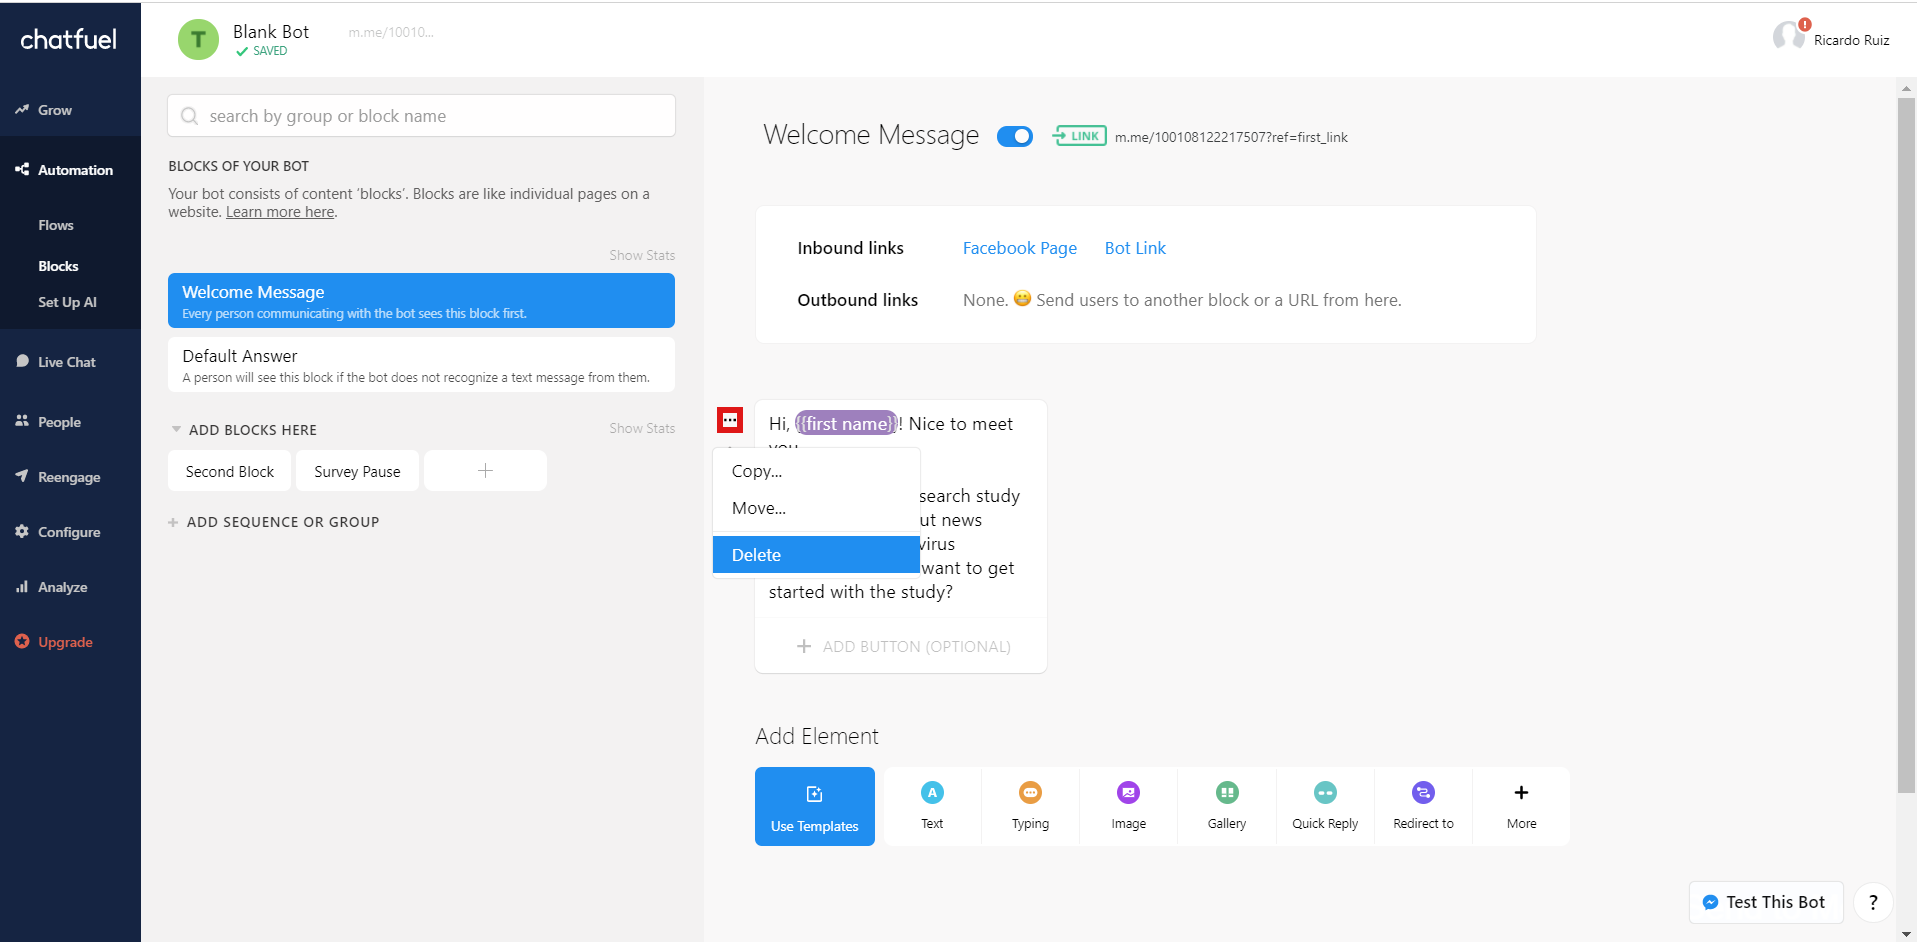
\includegraphics[scale=0.4]{assets/delete_card_redbox.PNG}}

\caption{Chatfuel: Delete Card}
\end{figure}


\subsubsection*{Redirecting }


To redirect to other blocks, we click on the More button in the add
elements section. Doing this takes us to the Chatfuel Plugins menu,
where we need to click on "Redirect to Block or Flow". Now we
will have a card that redirects to a block of our choice. We can also
conditionally redirect; in the example in Figure ?, we redirect individuals
with a timezone attribute of -7 UTC to the block titled, Second
Block.

\begin{figure}[H]
\center{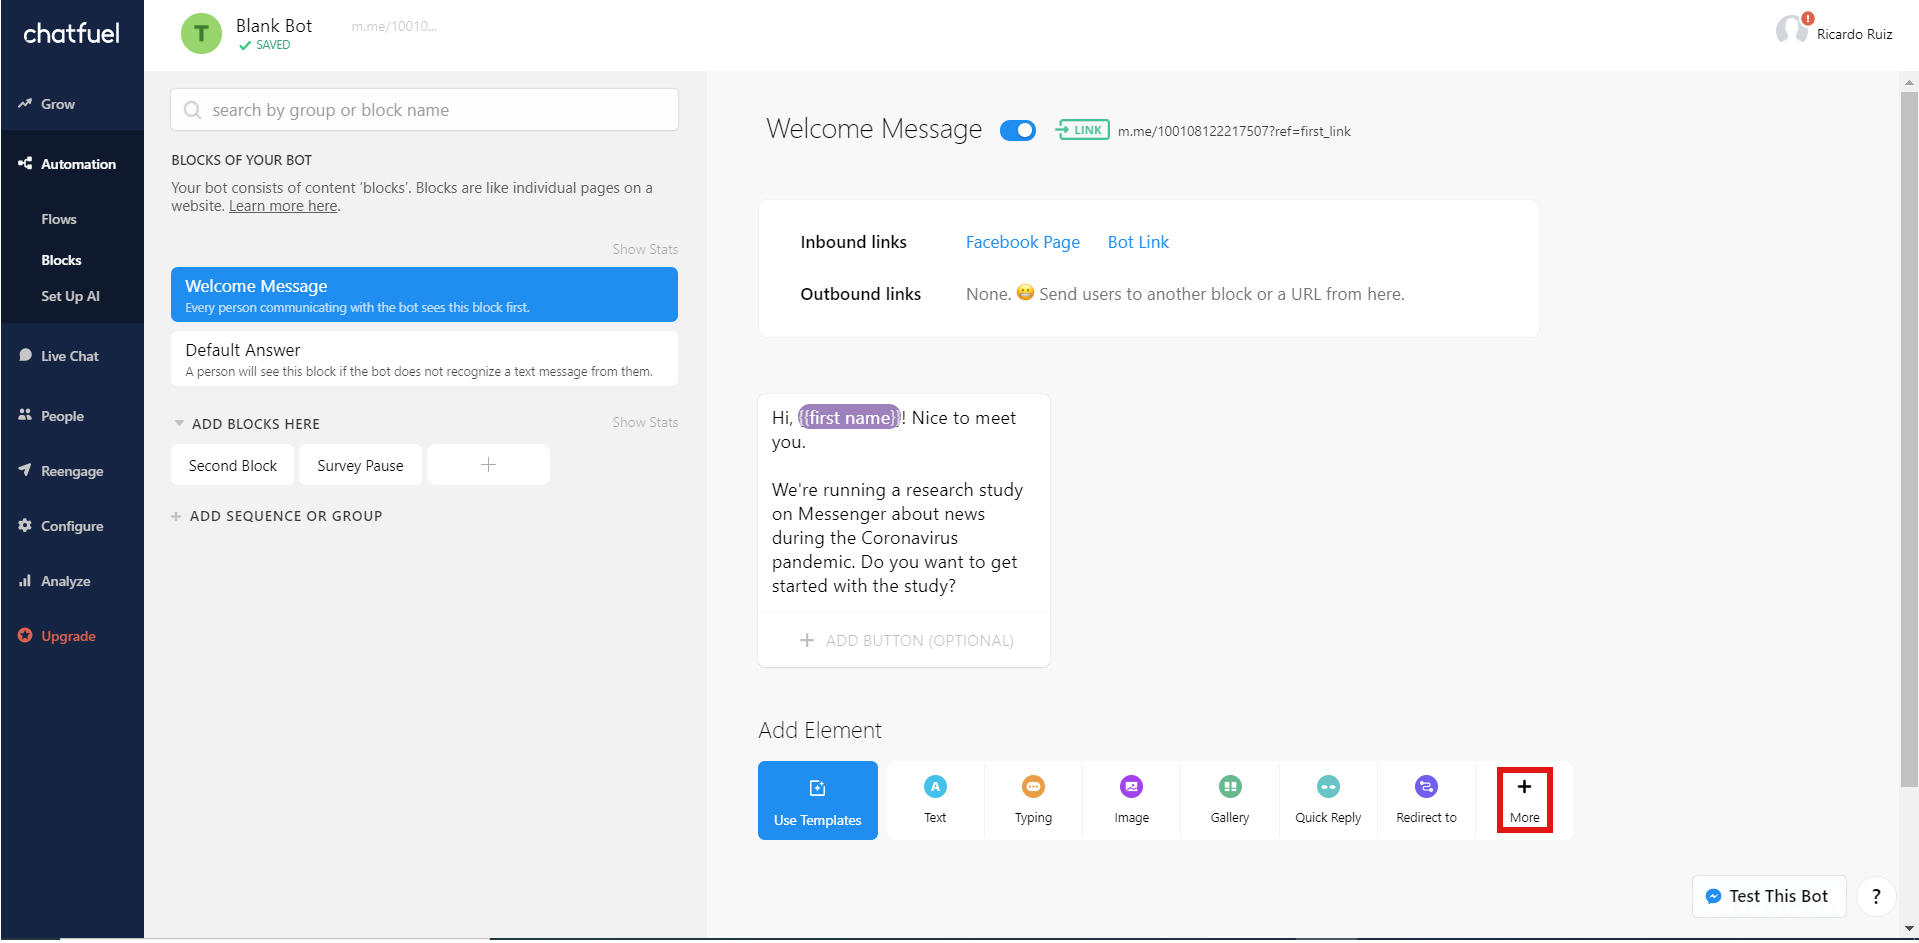
\includegraphics[scale=0.4]{assets/click_more_redbox.PNG}}

\caption{Chatfuel: More Button}
\end{figure}

\begin{figure}[H]
\center{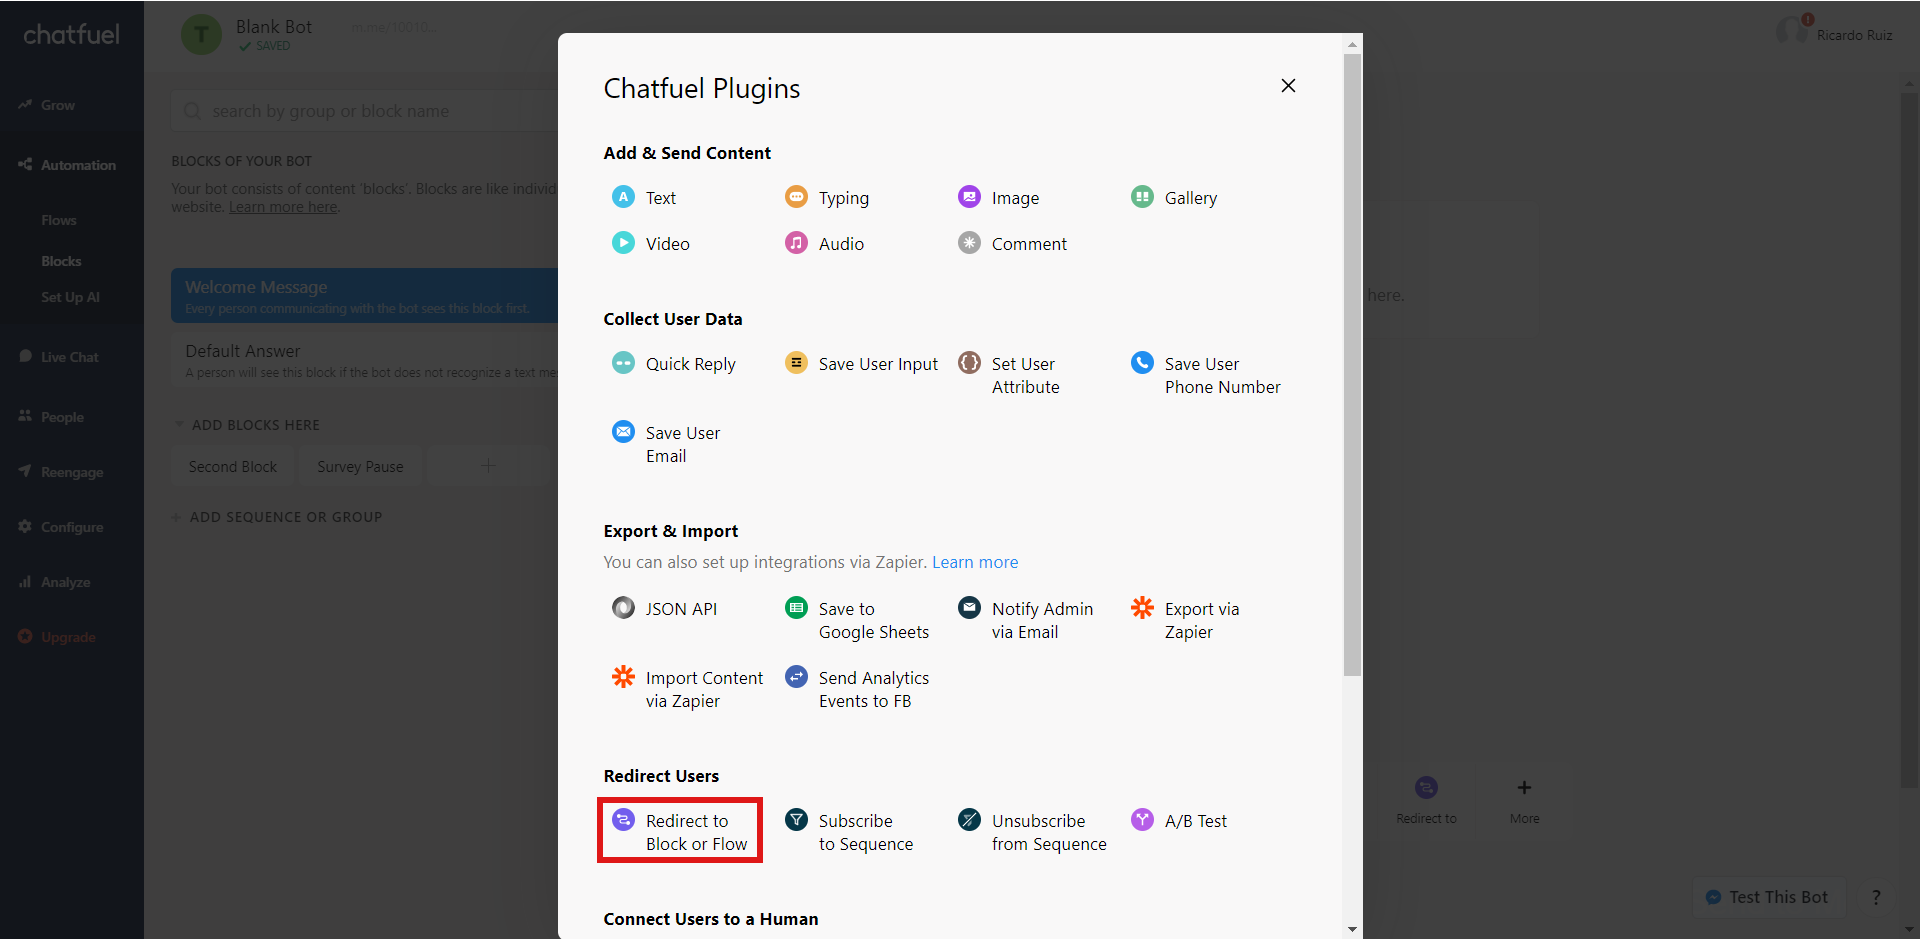
\includegraphics[scale=0.4]{assets/redirect_redbox.PNG}}

\caption{Chatfuel:Plugins Menu}
\end{figure}

\begin{figure}[H]
\center{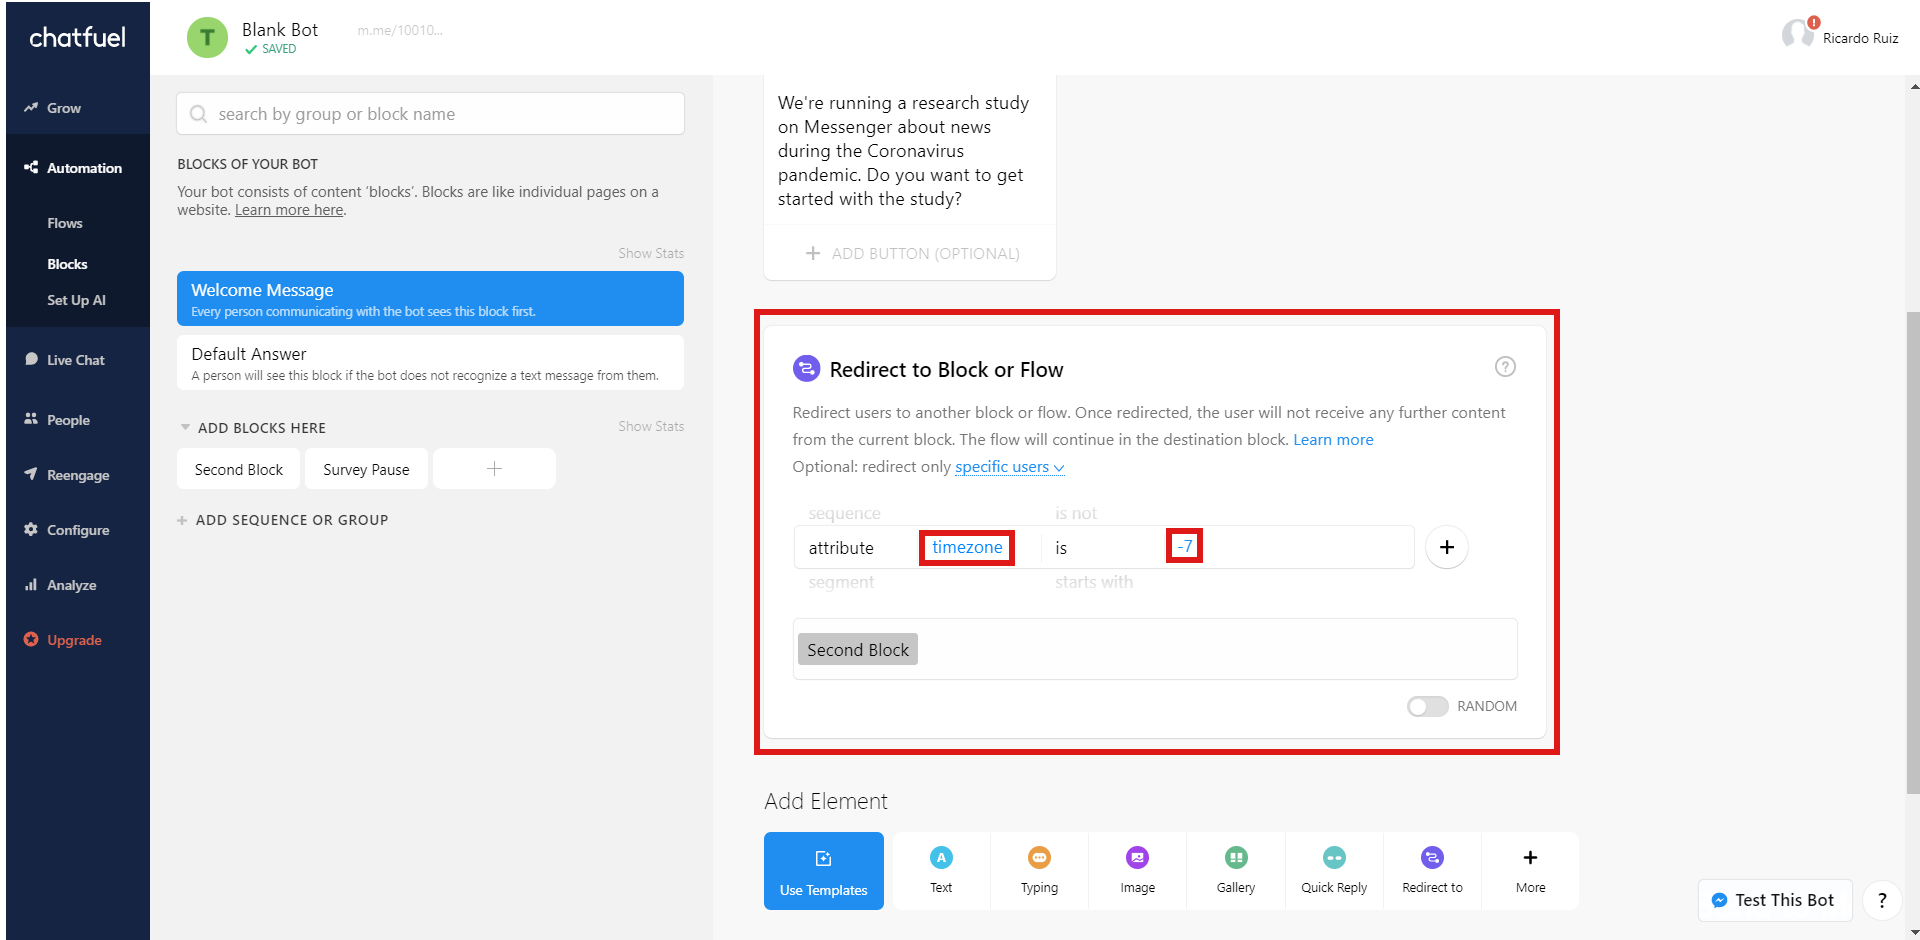
\includegraphics[scale=0.4]{assets/redirect_highlight_redbox.PNG}}

\caption{Chatfuel: Redirect}
\end{figure}


\subsubsection*{Setting User Attributes }

In the Chatfuel Plugins menu, you can select "Set User Attribute",
and input a name and value for the user attribute. Now any time an
individual passes this card, they will be assigned the specified attribute and value.  

\begin{figure}[H]
\center{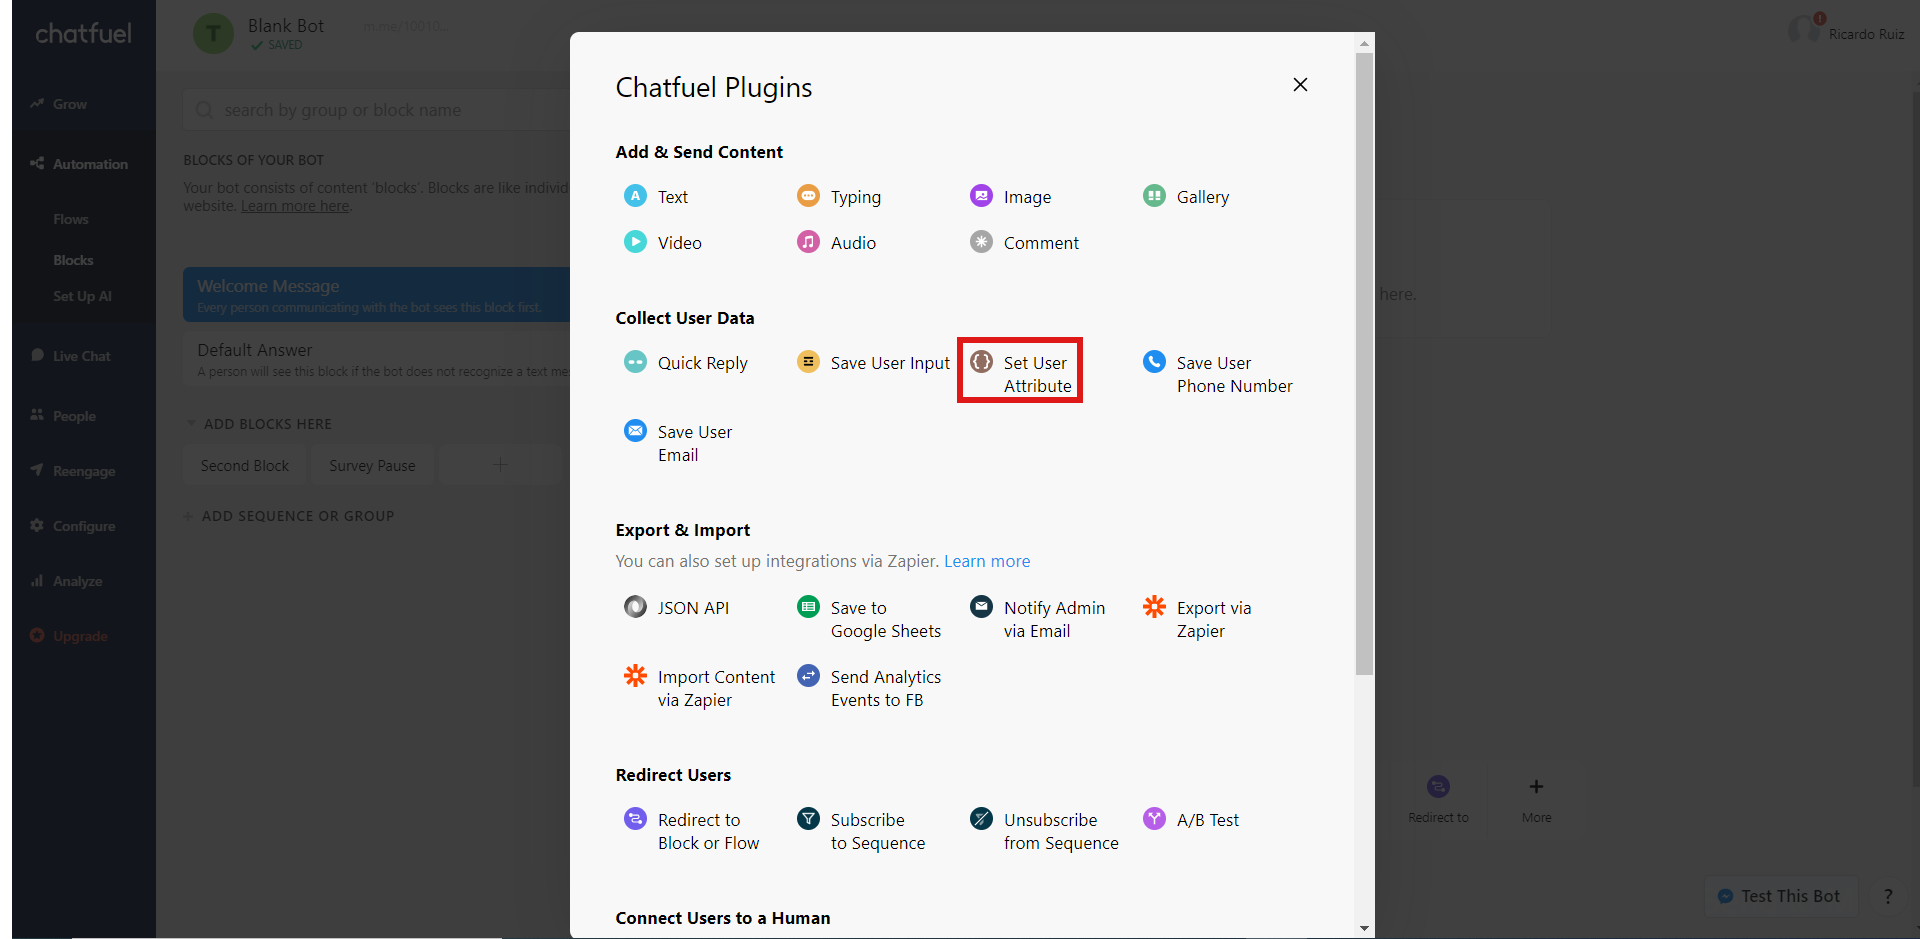
\includegraphics[scale=0.4]{assets/set_user_pick_redbox.PNG}}

\caption{Chatfuel: Set User Attributes}
\end{figure}

\begin{figure}[H]
\center{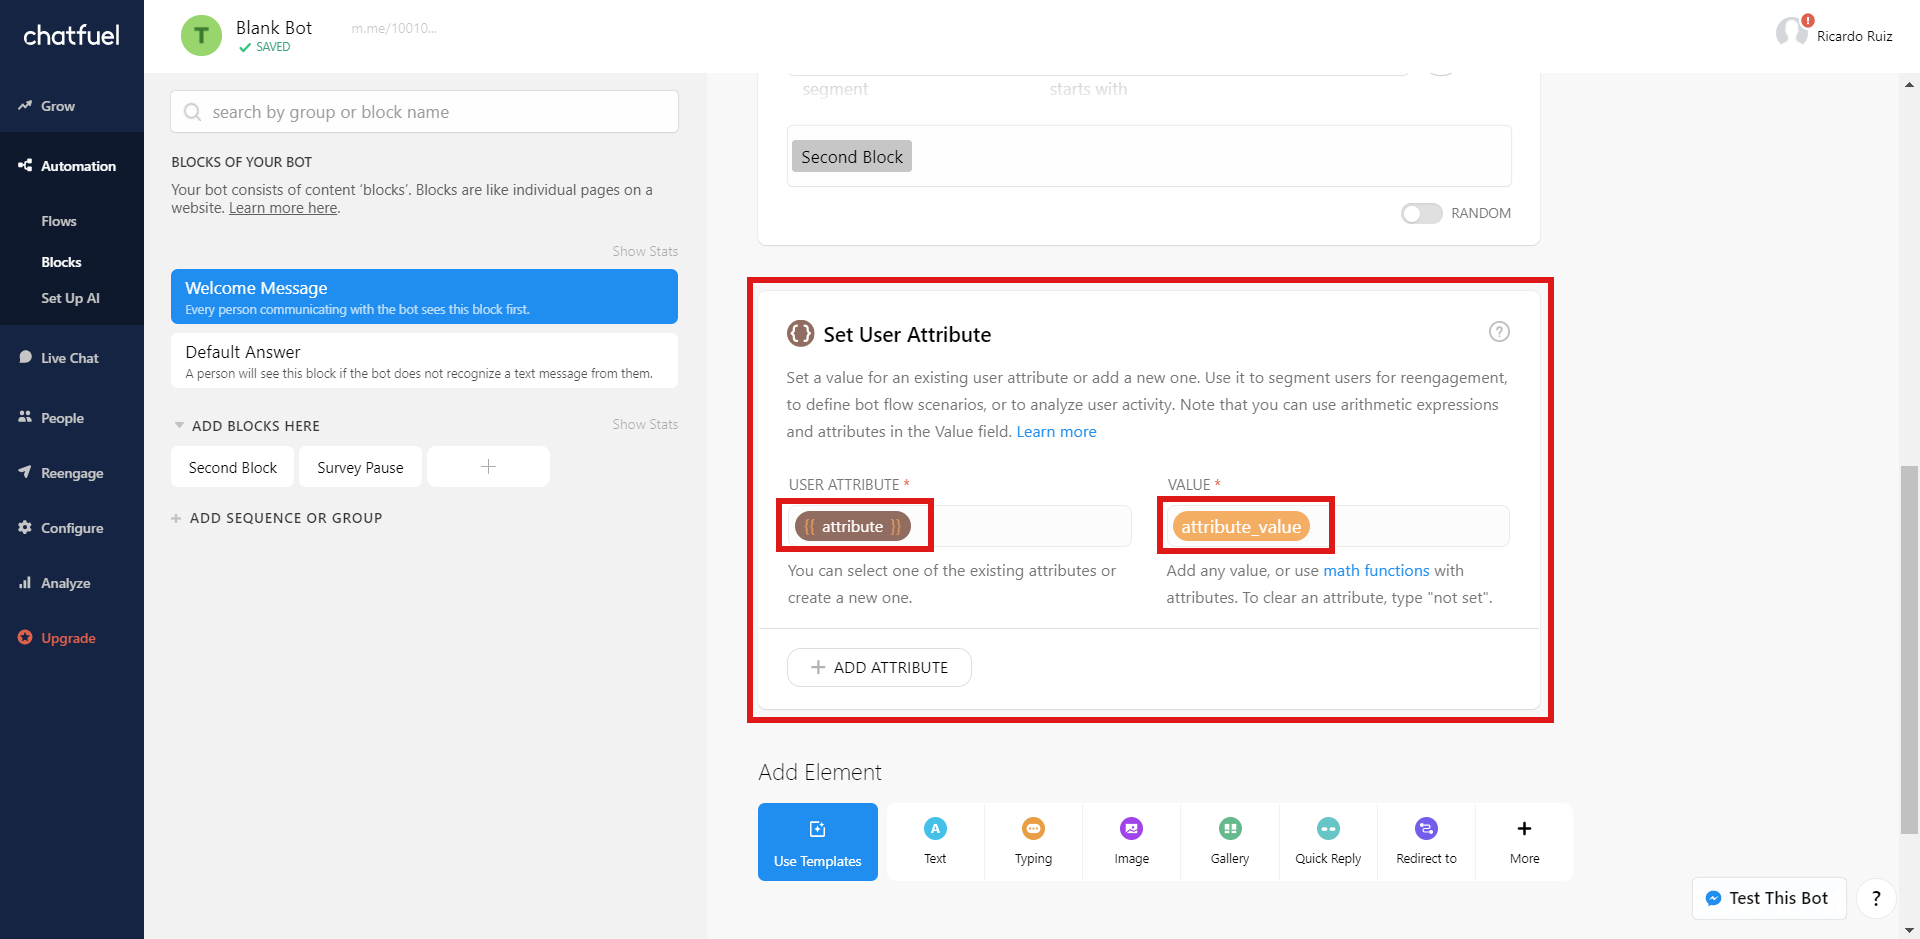
\includegraphics[scale=0.4]{assets/set_user_attributes_redbox.PNG}}

\caption{Chatfuel: Set User Attributes}
\end{figure}


\subsubsection*{Quick Replies }

After a text field, you can add a quick reply button, which gives
the user a button to respond to your text.

\begin{figure}[H]
\center{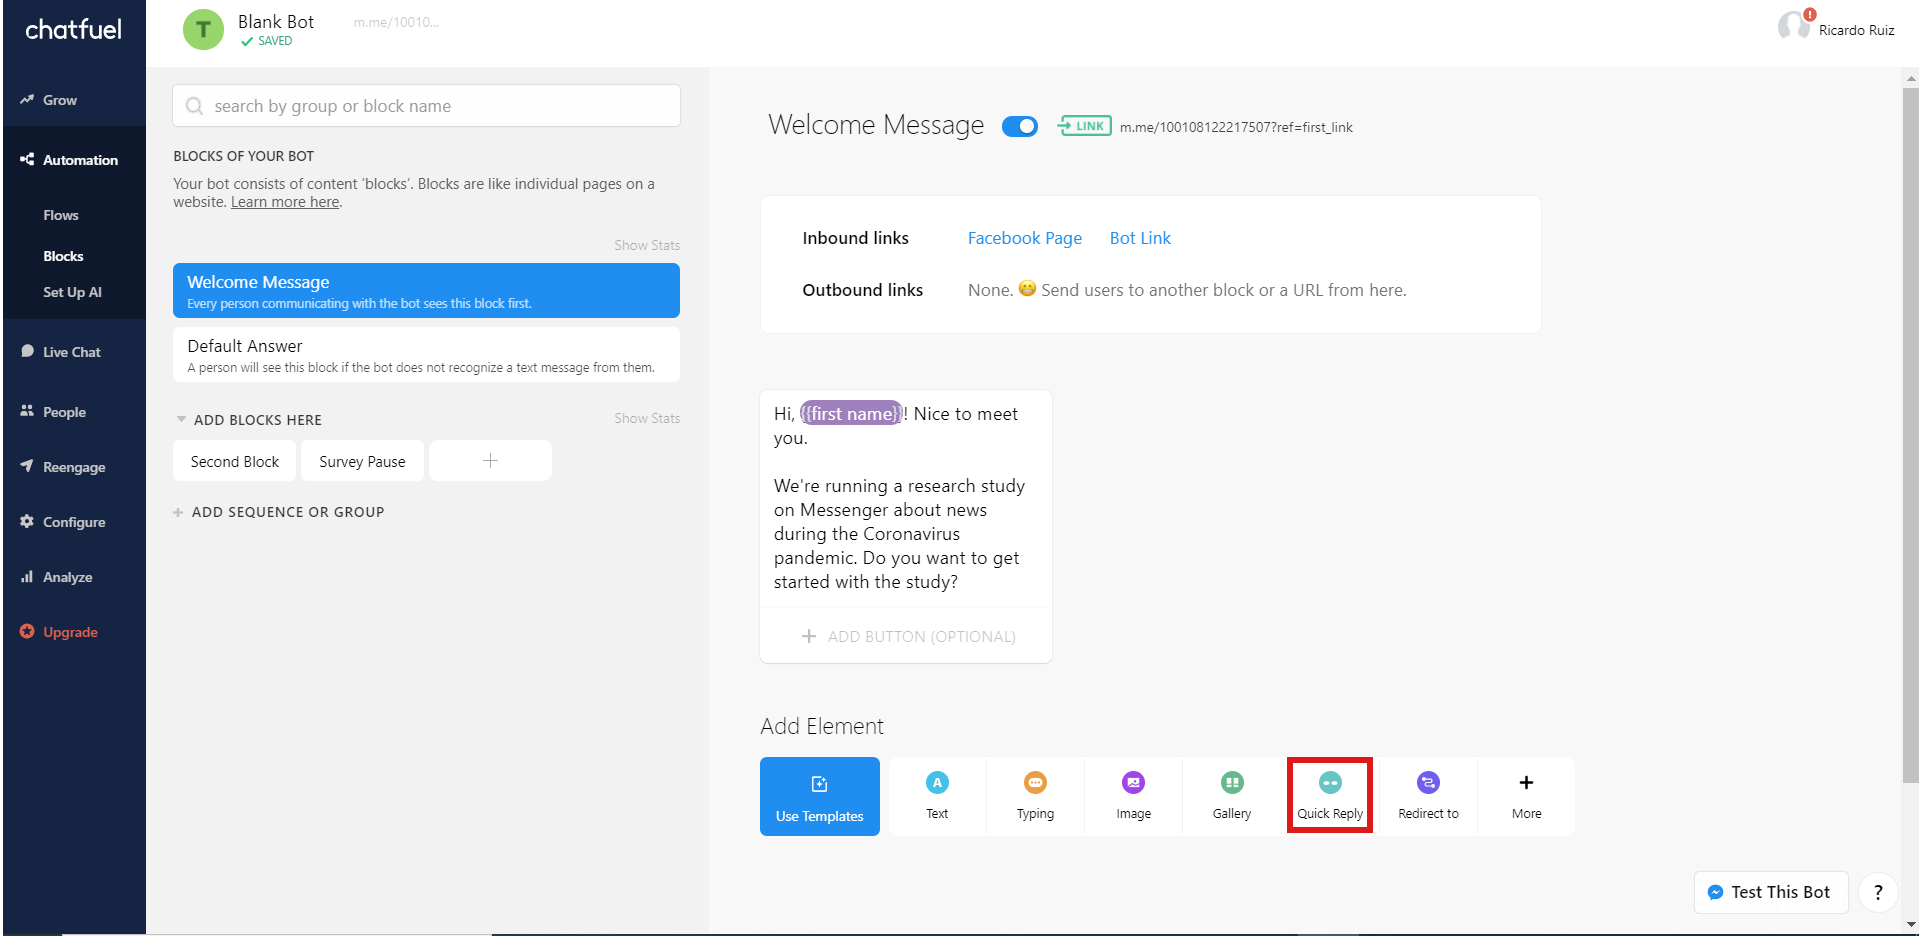
\includegraphics[scale=0.4]{assets/quick_reply_redbox.PNG}}

\caption{Chatfuel: Quick Reply}
\end{figure}

\begin{figure}[H]
\center{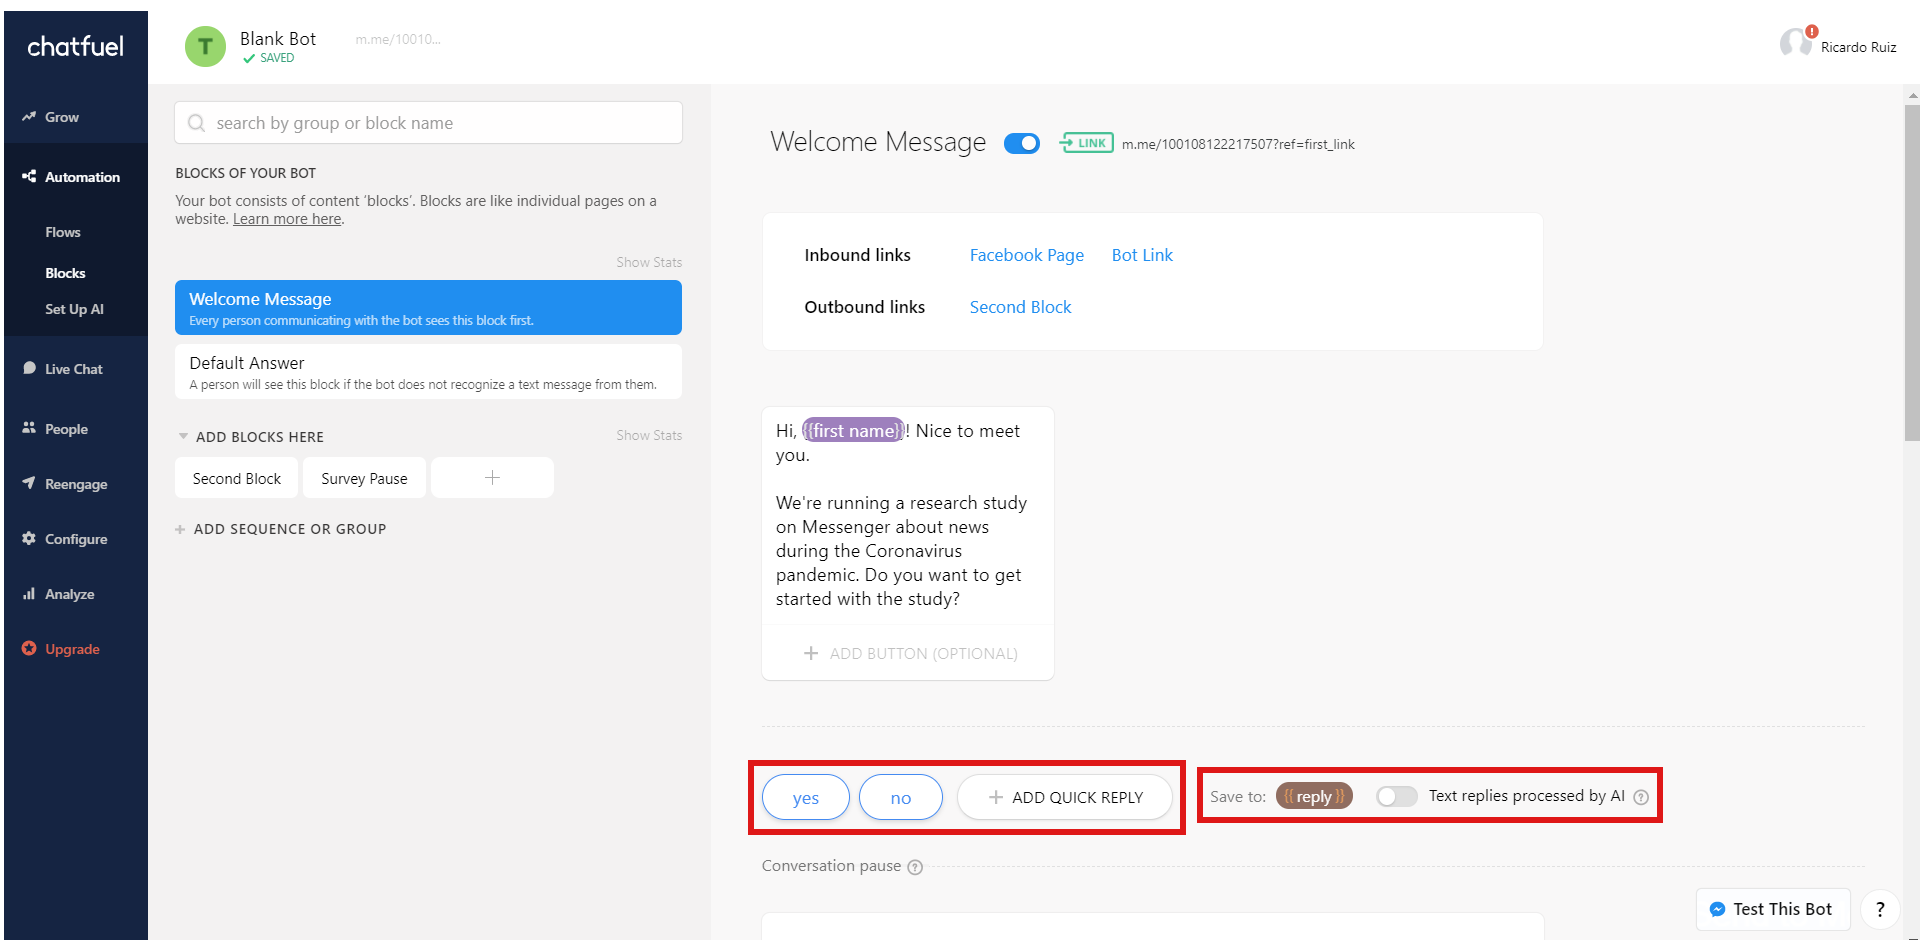
\includegraphics[scale=0.4]{assets/quick_reply2_redbox.PNG}}


\subsubsection*{Quick Replies }

After a text field, you can add a quick reply button, which gives
the user a button to respond to your text.

\caption{Chatfuel: Make Sure to turn off AI}
\end{figure}

That is the basics of building your chatbot, from here you will be
able to make and run your very first chatbot experiment! 


\subsubsection*{Random Redirects}

This will be used when assigning treatment uniformly at random. 


\subsection{During the Experiment}

During the experiment, the researcher must make sure that the chatbot
is functioning correctly. There will inevitably be some
sort of mistake/work-around that the individuals interacting with
the chatbot will find to go around some portion of your survey.
For instance, you might have inadvertently made it possible for individuals
to continue to the next block by inputting nonsense instead of responding yes or no. An example from the (misinformation experiment), even more severe than this, was when we had individuals attempting to get paid twice for participating in the experiment. If we hadn't been
actively watching over the bot, this could have been disastrous. The
good news is that when issues arise with your bot during the experiment,
you can fix them while the experiment is running! Simply go to the
block causing the problem and fix it. The two primary mechanisms you will be using to keep track of your chatbot are the people tab within Chatfuel and your Facebook page's inbox. You will see the individuals' assigned attributes in the experiment and download your data using the export button in the people tab. The inbox on your Facebook page will allow you to see all of the conversations the chatbot has had on your behalf. 

\begin{figure}[H]
\center{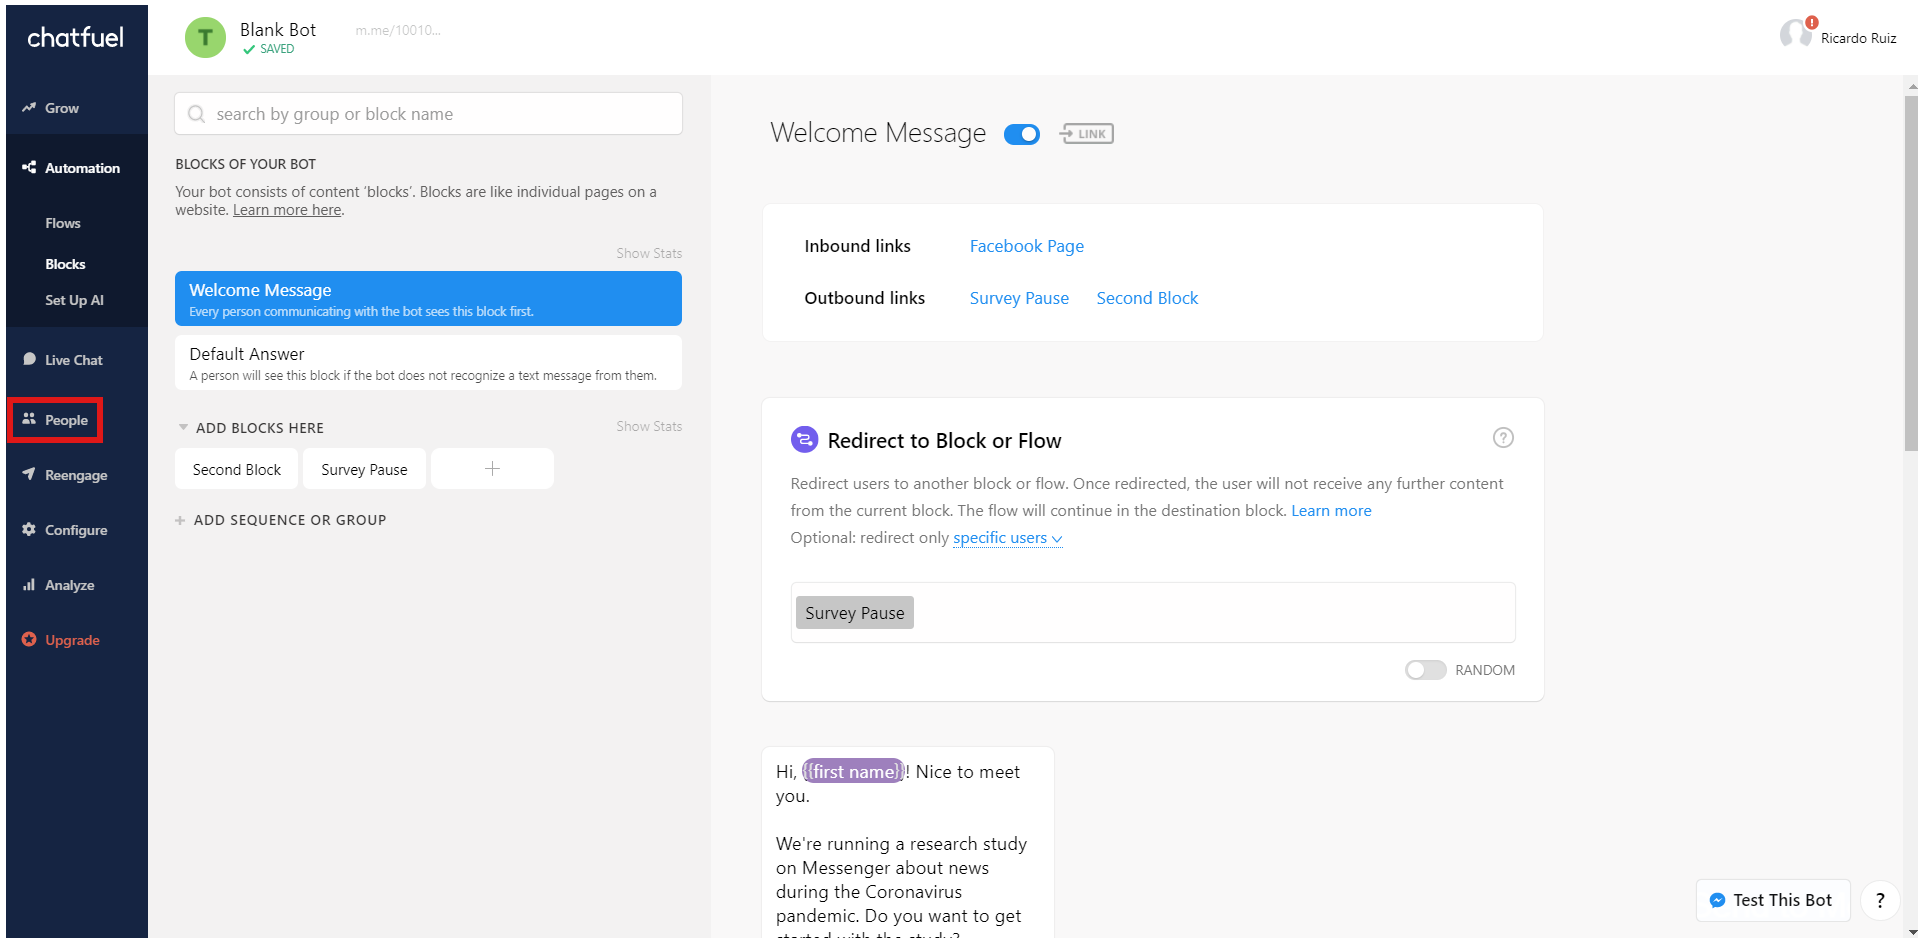
\includegraphics[scale=0.4]{assets/people_tab_redbox.PNG}}

\caption{Chatfuel: People Tab}
\end{figure}

\begin{figure}[H]
\center{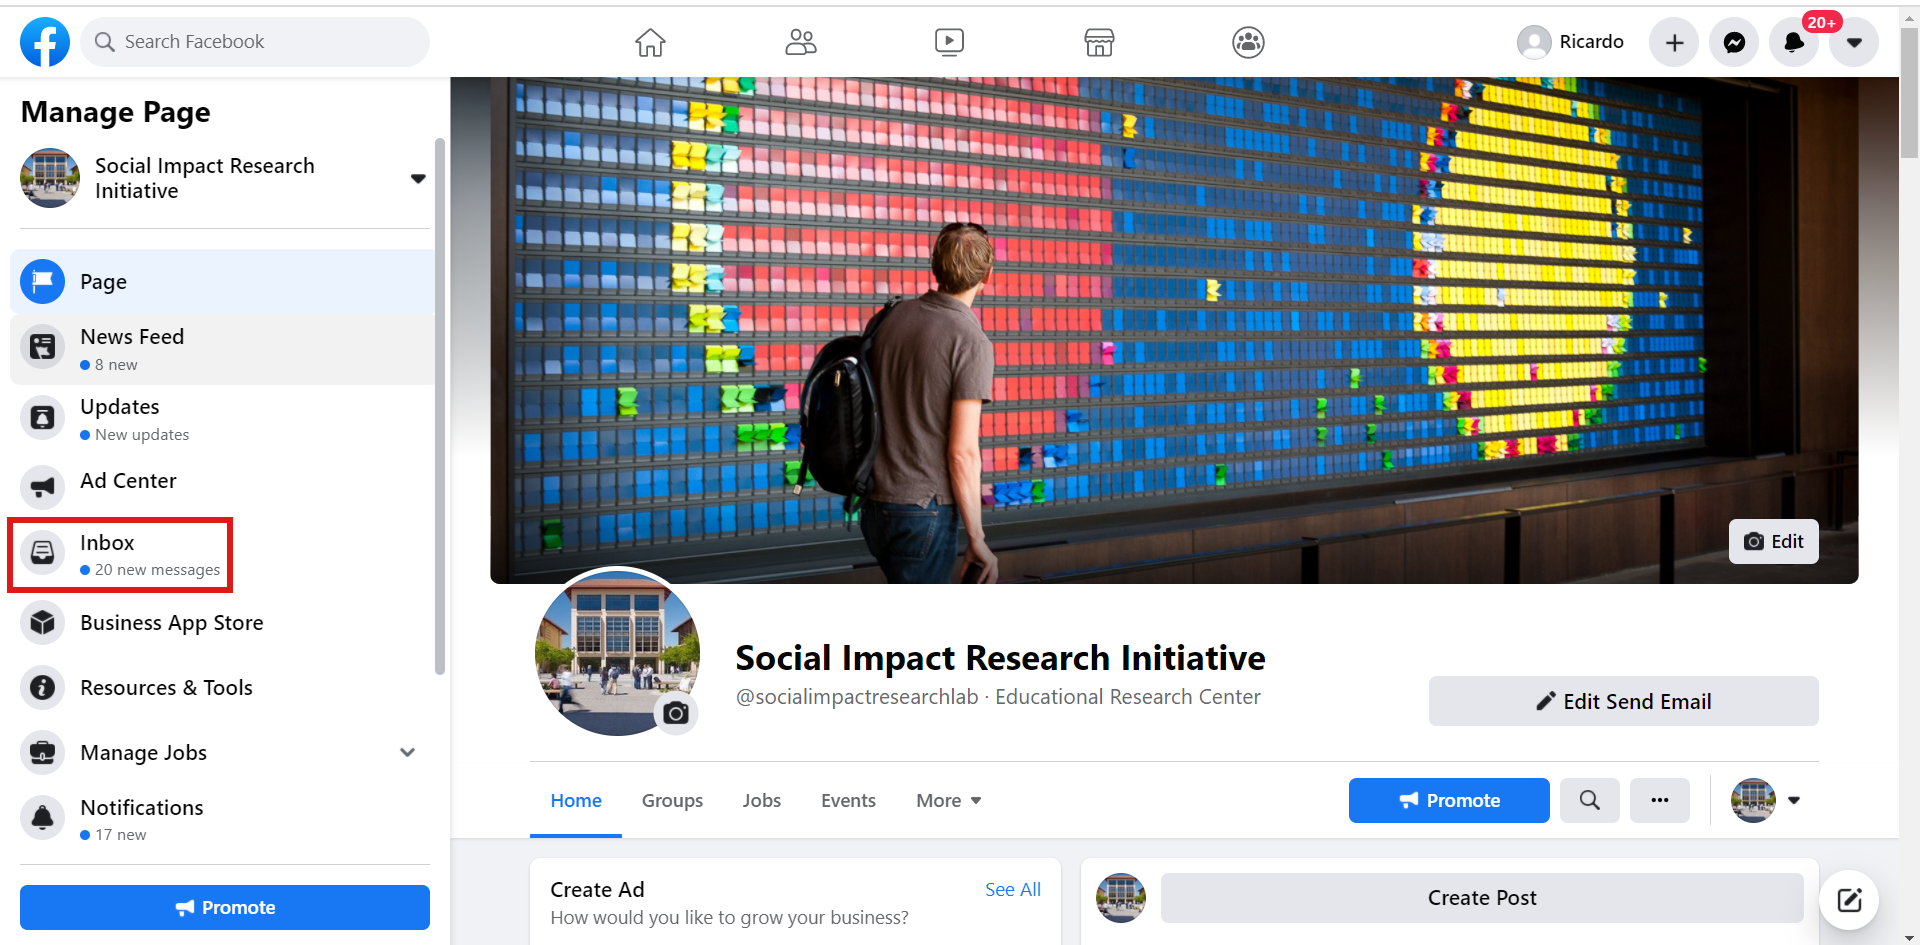
\includegraphics[scale=0.4]{assets/inbox_button_redbox.PNG}}

\caption{Facebook Page: Inbox}

\end{figure}

\begin{figure}[H]
\center{\includegraphics[scale=0.4]{to_make}}

\caption{Chatfuel: download data}

\end{figure}
\subsection{After the Experiment}

After the experiment, we must download the data as described above
and turn off the bot. The best practice for turning off the bot is
to insert a redirect to the pause block, as we described in the ``Before
the Experiment'' section. Doing this will allow individuals that
started the experiment to finish while simultaneously not allowing new
individuals to start the experiment. Finally, once you are satisfied
that all the individuals left in the experiment are done, you can
disconnect the chatbot from your Facebook page. The button is located in the Grow tab. 

\begin{figure}[H]
\center{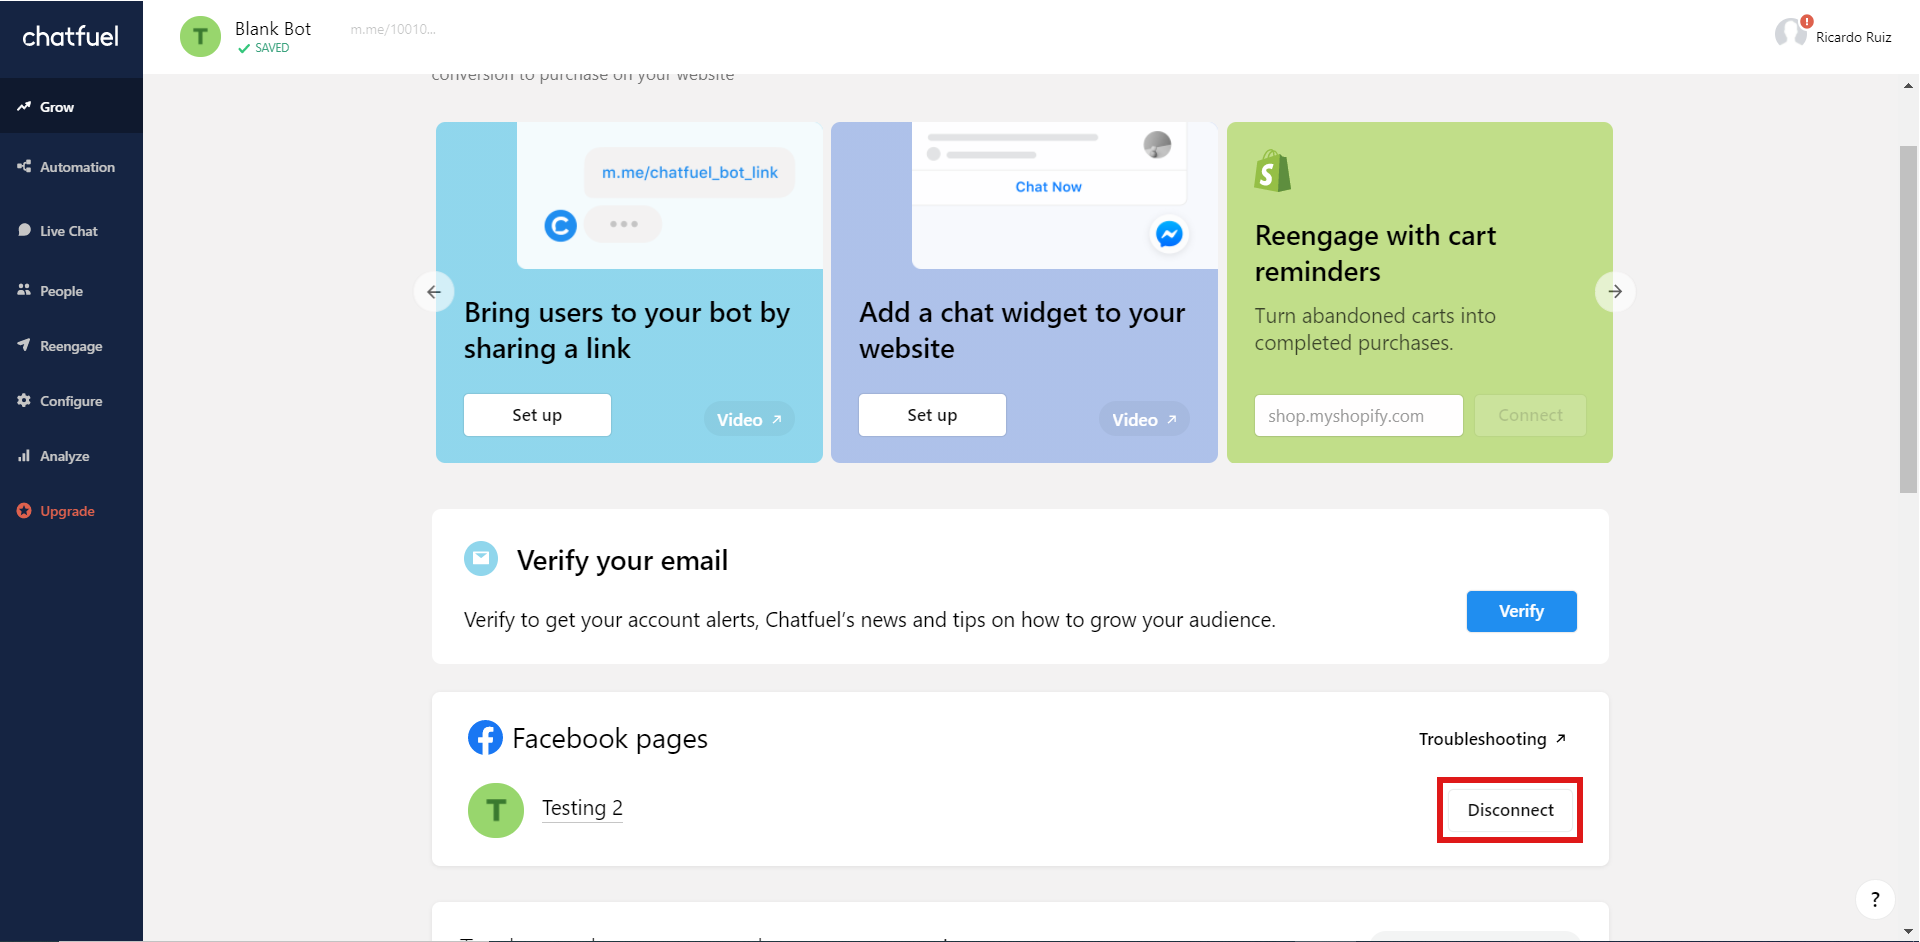
\includegraphics[scale=0.4]{assets/disconnect_bot_redbox.PNG}}

\caption{Disconnecting Chatbot}
\end{figure}


\section{The Adaptive Experiment Extension}

Now you might be wondering, can we extend this and run an adaptive experiment, perhaps even a contextual bandit? The great thing is that you can! To do so we have to setup an API, and have chatful interact with the API. This is easier than you might think. It will take some time to setup, but we will walk you through the steps. First we will begin by going over what needs to be changed on the Chatfuel side, and then we will go over setting up the server API. 

\subsection{The Adaptive Mechanism}
This is an outline of how a contextual or non-contextual bandit will function in our setup. Of note, a non-contextual bandit would start at step 2 and request treatment to be determined. 
\begin{enumerate}
    \item Obtain demographics information from chatfuel
    \item Send demographics information to server
    \item Server computes treatment according to model on server
    \item Chatfuel requests treatment
    \item Chatfuel uses returned treatment to assign treatment to user
    \item User udergoes treatment 
    \item Chatfuel sends results to the server
    \item Server updates model 
\end{enumerate}

\subsection{The Chatfuel Side}

\subsubseciton{Call the API}
We call the API using Chatfuel's JSON API plugin. Any time we wish to make some computation or retrieve some external information to Chatfuel, we will have to use this block. The highlighted web address will be the address to the server that we will set up in the next section. 

\subsubseciton{Using the API to randomize}

Once we receive our requested data from the API, we can use it within Chatfuel to redirect people to our treatment arms. It is important to note that Chatfuel will only wait for a response from the server for about 5 seconds. So, if your call to the API initiates a computation that takes longer than 5 seconds, you will need to make another call to the API to retrieve the result. 

Once you have received the treatment assignment of an individual from the API, you will need to use the following branching logic:  


\subsection{The Server Side}
Setting up the server side is much more complex, but we hope to seamlessly guide you through the process. We will go over how to setup the server using [heroku](heroku.com), however you can also host the server elsewhere such as Google App Engine, or even serverless using AWS.  
\begin{enumerate}

\item \textbf{Make an account on Heroku}


\item \textbf{Download the command line interface} 

Download the \href{https://devcenter.heroku.com/articles/heroku-cli}{command line interface} for your operating system. Currently supported operating systems are: MacOS, Windows, and Ubuntu.


\item \textbf{Fork Golub Github Repository}

Fork this repository which provides the basic file structure needed to setup the server, along with debugging information, and additional server help. You will insert your code to clean your data, determine treatment, send treatment, and update your model in your fork repository.

\item \textbf{Deploy code to heroku}

Follow the steps outlined \href{https://devcenter.heroku.com/articles/getting-started-with-python#deploy-the-app}{here} to deploy your app to the web. 

You will be given a url that we will use to interact with Chatufuel. 


Now your server is interacting with Chatfuel, and after you make the code to determine treatment, send treatment back, and update models; you will be able to run an adaptive expirement!
\end{enumerate}


\subsubsection{Additional Services}

There are two additional services that will come in handy. 


\begin{itemize}
    \item \textbf{Papertrail}
    
    This is a heroku addon that will log the output(stdout) from the server. 
    \item \textbf{hirefire.io}
    
    This is a third-party server scaling system that integrates with Heroku. It will only be needed if your code on the server is taking up to much of your allocated memory. 

\end{itemize}


\section{Advertising and Best Practices }

add section about qualtrics vs chatbot -{}-{}- somewhere 

add this to the end of setting up the bot 

Before we move on it is best practice to insert a redirect to a block
that pauses the survey whenever you don't want to collect any data.
This ensures that no one is able to interact with it when you aren't
running the expirement. To do this simply ... that redirects to a
message that .. . see Figure ? . 

Additionally, various aspects of the user expirence can be controlled
by the reseracher, from sending a daily message to setting a time
limit to complete the survey. 
\end{document}

